\chapter{Network monitoring with segment routing}
\label{chapter:scmon}


\section*{Introduction}

Monitoring is a crucial task for network operations. It is needed to ensure that all resources operate correctly (e.g., no
failures) and their configuration meets operator’s expectations (no congestion, required quality of service, etc.). Effective
monitoring is also fundamental for management tasks like traffic engineering, maintenance and troubleshooting.

\begin{figure}
\begin{center}
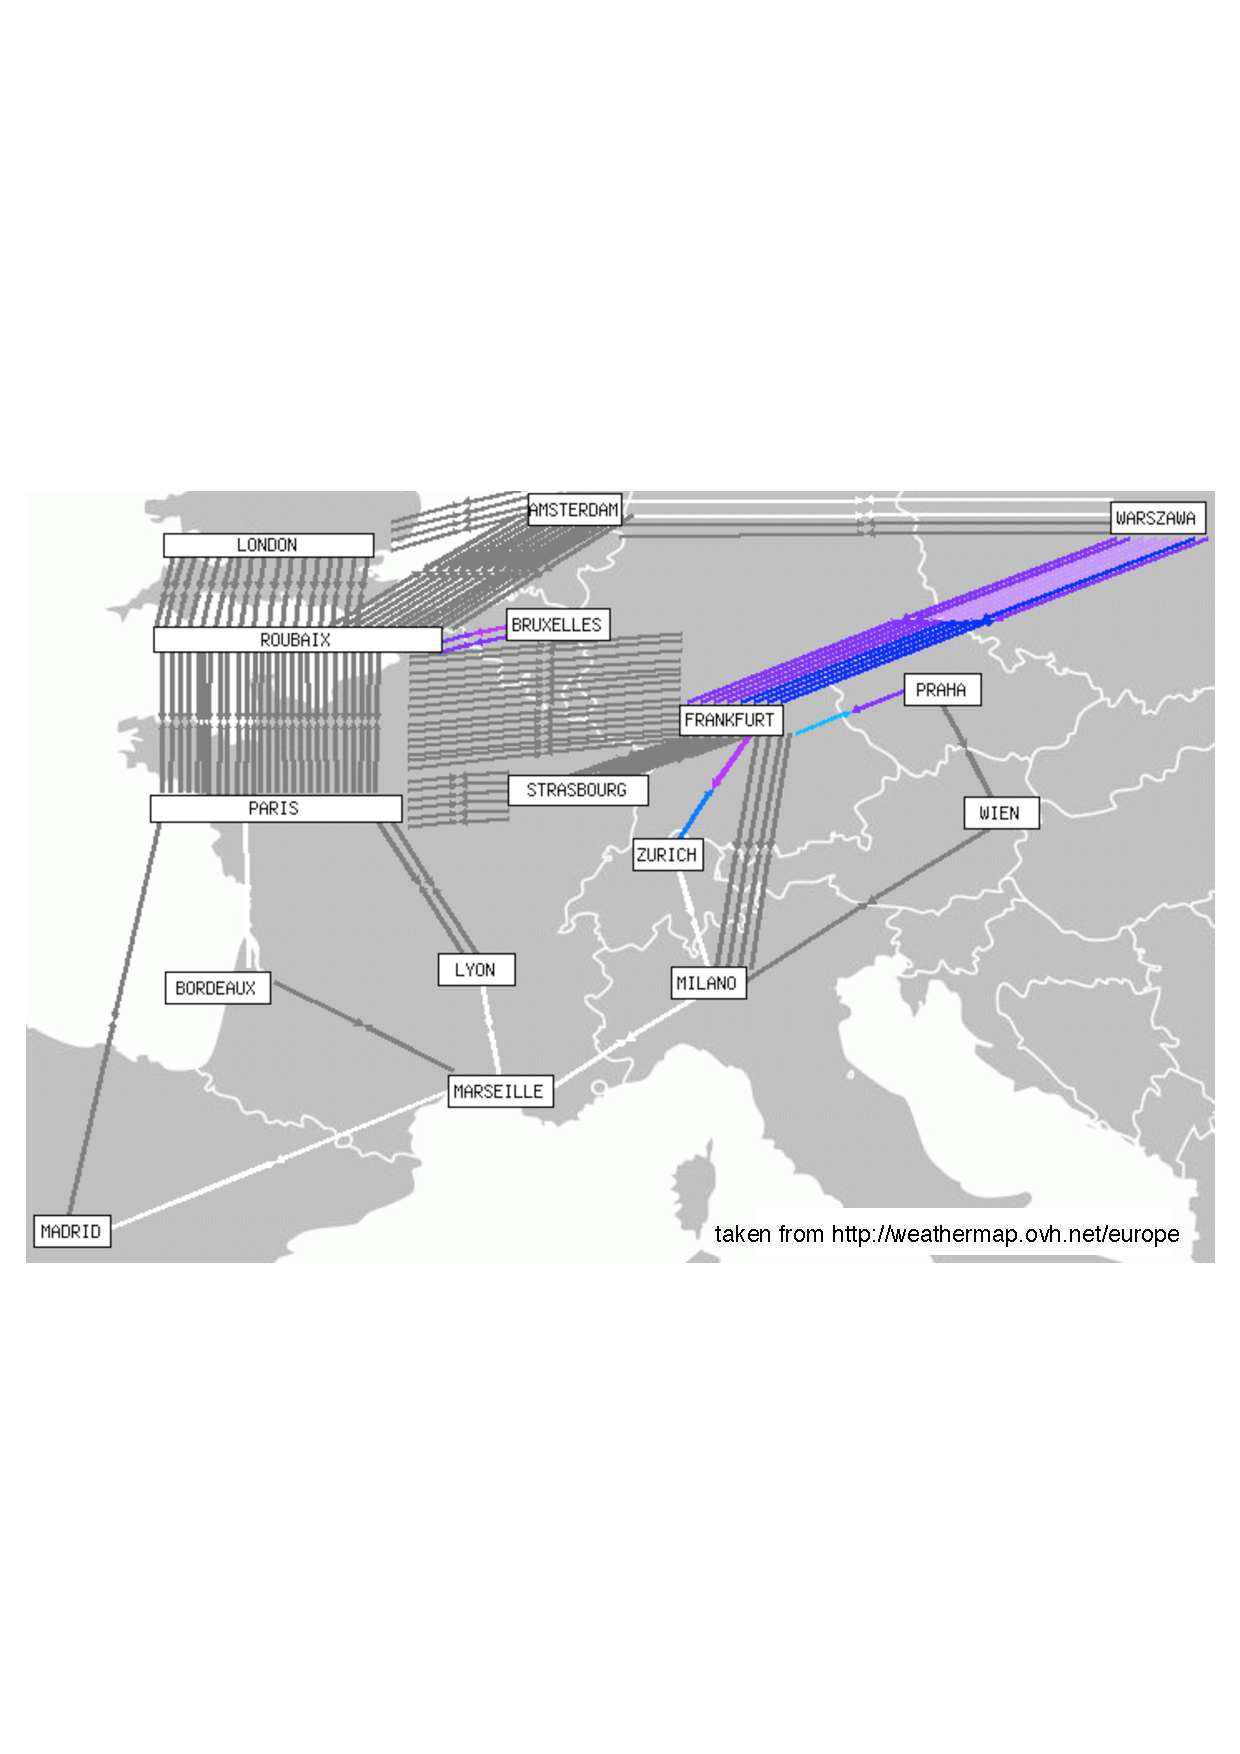
\includegraphics[width=.85\columnwidth]{figures/ovh-eu.pdf}
\end{center}
\caption{European backbone of \textsf{OVH}. In contrast to prior techniques, our algorithm can monitor health and performance of single
links in bundles (e.g., between \textsf{LONDON} and \textsf{ROUBAIX}).}
\label{fig:ovh}
\end{figure}


Unfortunately, even basic monitoring tasks, like checking for hardware malfunctions, are practically hard, due to the
complexity of current networks. Prominently, multi-path routing is widely used, both to spread the load on multiple paths
and to aggregate parallel links in bundles.
Figure \ref{fig:ovh} shows an overview of the European backbone of a big cloud provider,
\textsf{OVH}. It highlights that parallel links are used at the same time between many pairs of routers. While enabling better
performance and robustness, multi-path routing also poses significant obstacles to monitoring. For instance, assessing
the exact path and performance of each packet becomes complex [2], [20] since such a path depends on (vendor-specific) hash functions used by routers for load-balancing.

As a consequence, not only naive approaches (e.g., based on ping or traceroute) are not sufficient, but also 
state-of-the-art monitoring techniques tend to be ineffective.


On the one hand, protocol-based approaches use control-plane messages to infer possible failures. 
For example, link-state routing protocols (like OSPF or IS-IS) or specialized
ones (BFD [14]) rely on heartbeat-like mechanisms to check
bi-directional connectivity among pairs of adjacent nodes. This
approach only ensures detection of failures that affect control plane messages. 
However, it cannot be used to detect failures that only affect data-plane traffic like: 

\begin{enumerate}[i)]
\item corruption of an
optical link that leads to framing errors and packet losses;
\item malfunctioning of a router interface that considers the link still up but discards all the received packets;
\item failure of only one link among the parallel ones between two routers.
\end{enumerate}

On the other hand, probe-based techniques rely on sending
data-plane monitoring packets, i.e., probes, between fixed
vantage points in the network. Vantage points typically run
standard protocols (e.g., IPSLA [8]) to send probes and extract
measurements from them. Unfortunately, if the probes are sent
over paths used to forward regular traffic, many vantage points
may be needed to obtain high coverage, and links not used
by current paths (e.g., backup links) cannot be checked at
all. Otherwise, probes can be sent over tunnels (e.g., RSVP-TE [3] ones) to enforce specific paths, but this is not scalable.
Indeed, even for detecting single-link failures and pinpointing
their position, the number of needed tunnels tends to explode,
and so does the control-plane overhead (to signal tunnels) [7].

We propose a new technique that ensures full coverage of all network resources from a
single vantage point. It is based on sending data-plane probes over carefully-chosen cycles. This way, a single box can both
send and receive monitoring probes, avoiding the need for synchronizing and coordinating multiple vantage points, hence
minimizing infrastructural costs. By relying on data-plane measurements, we support both detection of hardware failures and resource overloading (e.g., link congestion).

% Segment routing generates conflicting objectives for the computation
% of cycles over which probes are sent. On the one hand, we would like to minimize the number of cycles, to reduce the
% monitoring overhead; hence, we should have cycles that are long and few in number. On the other hand, we need cycles
% to be enforced in practice, and long cycles may require too many segments even for the most powerful commercial routers
% (currently supporting less than 10 segments). To tackle those challenges, SCMon runs original algorithms
% that compute cycles on a monitoring topology, maintained by routers in addition to the one used for user traffic. The monitoring topology spans all network links, 
% and uses carefully computed weights that avoid (as much as possible) ECMP paths, i.e., multiple shortest paths between a pair of nodes.
% Note that existing routers have already been shown to well support two topologies and their (limited) overhead [17].
% SCMon supports detection and localization of any set of link failures/overloading. It infers single-link failures by keeping
% track of the cycles associated to probes sent and not received at the monitoring box. For multiple link failures, we have two
% cases. Some of them, e.g., affecting links in disjoint cycles, are detected directly from the set of lost probes (as single-link failures). 
% The others, e.g., affecting two links belonging to a single monitoring cycle, are reported by SCMon one at
% a time: This provides operators with a debugging interface (asking to correct one error before showing another one)
% similar to the one of a compiler for software programs. Similar considerations apply to node failures and link congestion.
% In developing SCMon, we make three main contributions.
% 
% Our approach to compute monitoring cycles consists of four steps.
% The first step computes IGP weights for the monitoring topology, in order to minimize ECMP paths.
% The second step models link bundles aggregated into a single IGP link. 
% The third step calculates a set of cycles covering the whole network and sharing the node from which probes are sent.
% The last step computes the SR segments to send probes over those cycles.


%In this section we will propose several algorithms and strategies to compute a cycle cover of the network
%using segment routing. We need however to impose some properties in the cycle cover in order to be able to use
%it for detecting single link failures in a network. Those properties as the following:

As usual, we start by defining the problems that we tackle in this chapter. To do that we need the two following definitions.
Throughout this chapter we assume that the network topology is symmetric.

\begin{definition}
Let $G$ be a symmetric network, $s \in V(G)$ and $k \in \mathbb{N}$. We denote by $\mathcal{C}^k_s$ the set of deterministic sr-cycles from $s$ to $s$ with segment cost at most $k$.
\end{definition}

\begin{definition}
Let $G$ be a symmetric network, $s \in V(G)$ and $k \in \mathbb{N}$. A \emph{$k$ sr-cycle cover} of a network $G$ 
with vantage point $s$ is a subset $C \subseteq \mathcal{C}^k_s$ of deterministic sr-cycles such
that for each edge $e \in E(G)$ there exists $\sr{c} \in C$ such that $e \in E(\sr{c})$.
\end{definition}

Below we define the two problems that we tackle in this chapter. Both of them seek to compute a cycle cover.
The first aims at minimizing the maximum segment cost of any sr-cycle in the cover while the second wants to minimize the number of cycles for a given segment cost limit.
% We will see that the first problem admits a polynomial time solution and that the second one is \NPhard.


\begin{problem}{Min segment cost cover}
\label{prob:min-seg-cover}
\textbf{Input:} A symmetric network $G$ and $s \in V(G)$.

\textbf{Output:} A sr-cycle cover $C$ of $G$ such that the maximum segment cost of any sr-cycle $\sr{c} \in C$ is minimum.
\end{problem}

\begin{problem}{Min sr-cycle cover}
\label{prob:min-cycle-cover}
\textbf{Input:} A symmetric network $G$, $s \in V(G)$ and $k \in \mathbb{N}$.

\textbf{Output:} A sr-cycle cover $C \subseteq \Csk$ of $G$ such that $|C|$ is minimum.
\end{problem}
% 
% \begin{proposition}
% Problem \ref{prob:min-cycle-cover} is \NPhard.
% \end{proposition}
% 
% \begin{proof}
% The problem of finding a minimum cardinaly cycle cover of a graph is \NPhard and by setting $k$
% large enough and setting IGP weights such that there is not ECMP any solution
% to Problem \ref{prob:min-cycle-cover} corresponds to a minimum cycle cover.
% \end{proof}
% 


\section{Minimum segment cost covers}

In this section we propose a polynomial time algorithm for solving Problem \ref{prob:min-seg-cover}.
We have seen in Chapter \ref{chapter:sr} reachability results that tells us exactly how costly,
in terms of segments, it is to deterministically reach a given node in the network. Using these results
we can easily establish how costly it is to cover a given edge with a deterministic sr-cycle.

In order to cover a given edge $e$ with a deterministic sr-cycle from $s$ to $s$ with segment cost at most
$k$, we have essentially two options:

\begin{enumerate}
 \item First we go from $s$ to some node $x$ using a deterministic sr-path of cost, say, $k_1$. Then travel
 from $x$ to some node $y$ via a unique shortest path that contains edge $e$. Finally, we go from $y$ back to $s$
 with a deterministic sr-path of cost $k_2 = k - k_1$. This is illustrated in Figure \ref{fig:cover-edge1}.
 
\begin{figure}
\begin{center}
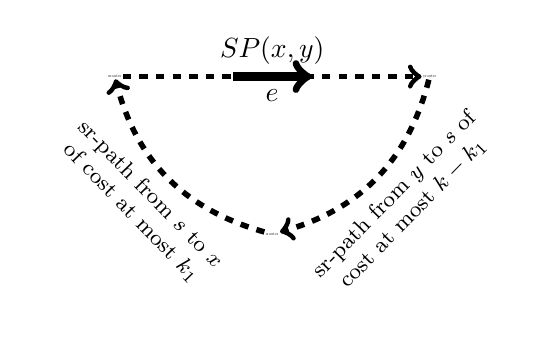
\begin{tikzpicture}
\def\x{0}
\def\y{0}

\node[scale=0.15] (s) at (0 + \x, 0 + \y)  {\router{s}{router}};
\node[scale=0.15] (x) at (-2 + \x, 2 + \y) {\router{x}{router}};
\node[scale=0.15] (y) at (2 + \x,  2 + \y) {\router{y}{router}};

\draw[line width=2, black] (s) edge[below, sloped, bend left, dashed, ->] node[black] {
\footnotesize
\begin{tabular}{c}
 sr-path from $s$ to $x$ \\
 of cost at most $k_1$
\end{tabular}
} (x);
\draw[line width=2, black] (y) edge[below, sloped, bend left, dashed, ->] node[black] {
\footnotesize
\begin{tabular}{c}
 sr-path from $y$ to $s$ of \\
 cost at most $k - k_1$
\end{tabular}
} (s);

\draw[line width=2, black] (x) edge[above, sloped, dashed, ->] node[black,font=\bfseries] {\texttt{$SP(x, y)$}} (y);

\draw[line width=3] (-0.5, 2) edge[below, ->] node {$e$} (0.5, 2);

\end{tikzpicture}
\end{center}
\caption{First case of edge covering.}
\label{fig:cover-edge1}
\end{figure}

 
 \item The second way to cover $e$ is to use an adjacency segment over it. To do so, we first go from $s$ to
 some node $x$ with a deterministic sr-path of cost at most, say, $k_1$. This node $x$ must be such that it contains 
 a unique shortest path to $e^1$. Otherwise the resulting cycle would not be deterministic. Then we use an adjacency 
 segment on $e$ to traverse it by following the unique shortest path between $x$ and $e^1$ and then $e$.
 Then we go to some node $y$ via a unique shortest path from $e^2$. Finally, we go from $y$ back to $s$ with a
 sr-path of cost at most $k_2 = k - k_1 - 2$. The $-2$ comes from the fact that we spent a segment cost of $2$ 
 with the adjacency segment $e$. This case is illustrated in Figure \ref{fig:cover-edge2}.

\begin{figure}
\begin{center}
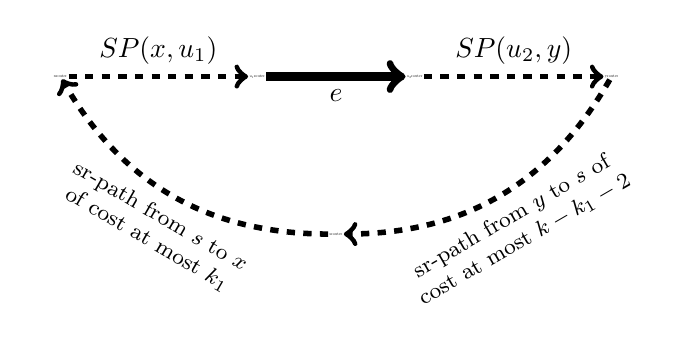
\begin{tikzpicture}
\def\x{0}
\def\y{0}

\node[scale=0.15] (s) at (0 + \x, 0 + \y)  {\router{s}{router}};
\node[scale=0.15] (x) at (-3.5 + \x, 2 + \y) {\router{x}{router}};
\node[scale=0.15] (y) at (3.5 + \x,  2 + \y) {\router{y}{router}};
\node[scale=0.15] (u1) at (-1 + \x,  2 + \y) {\router{$u_1$}{router}};
\node[scale=0.15] (u2) at (1 + \x,  2 + \y) {\router{$u_2$}{router}};

\draw[line width=2, black] (s) edge[below, sloped, bend left, dashed, ->] node[black] {
\footnotesize
\begin{tabular}{c}
 sr-path from $s$ to $x$ \\
 of cost at most $k_1$
\end{tabular}
} (x);
\draw[line width=2, black] (y) edge[below, sloped, bend left, dashed, ->] node[black] {
\footnotesize
\begin{tabular}{c}
 sr-path from $y$ to $s$ of \\
 cost at most $k - k_1 - 2$
\end{tabular}
} (s);

\draw[line width=2, black] (x) edge[above, sloped, dashed, ->] node[black,font=\bfseries] {\texttt{$SP(x, u_1)$}} (u1);
\draw[line width=2, black] (u2) edge[above, sloped, dashed, ->] node[black,font=\bfseries] {\texttt{$SP(u_2, y)$}} (y);


\draw[line width=3] (u1) edge[below, ->] node {$e$} (u2);

\end{tikzpicture}
\end{center}
\caption{Second case of edge covering.}
\label{fig:cover-edge2}
\end{figure} 
\end{enumerate}

Note that in both cases, nothings prevents us to have $x = e^1$ or $y = e^2$. We do not require these nodes to be distinct
as doing so would provide an incomplete description of all possible cases.

Next we prove formally that those two cases cover all possibilities. The next theorem directly translate into
a polynomial time algorithm for computing minimum segment cost covers.

\begin{theorem}
\label{thm:edge-cover}
Let $G$ be a network $s \in V(G)$, $e \in E(G)$ and $k \in \mathbb{N}$ an integer. There exists a deterministic sr-cycle $\sr{c}$
from $s$ to $s$ of cost at most $k$ such that $e \in E(\sr{c})$ if and only if there exist integers $k_1, k_2 \geq 1$, $x \in \nreach(k_1, s)$, $y$ such that $s \in \nreach(k_2, y)$ 
and one of the two following conditions holds
\begin{enumerate}[(1)]
 \item $k_1 + k_2 = k$, $y \in \spreach(x)$ and $e \in \sp(x, y)$
 \item $k_1 + k_2 = k - 2$, $e^1 \in \spreach(x)$ and $y \in \spreach(e^2)$
\end{enumerate}
\end{theorem}

\begin{proof}
Let $G$ be a network $s \in V(G)$, $e \in E(G)$ and $k \geq 1$ an integer.

$(\Rightarrow)$ Assume that there exists a deterministic sr-cycle $\sr{c}$ from $s$ to $s$
with $\cost(\sr{c}) \leq k$ such that $e \in E(\sr{c})$. Write $\sr{c} = \langle x_1, \ldots, x_l \rangle$.
Since $e \in E(\sr{c})$ there exists $i \in \{1, \ldots, l\}$ such that either $x_i = e$ or $i < l$ and
$e \in \sp(x^2_{i}, x^1_{i + 1})$.

\emph{Case 1:} $e \in \sp(x^2_{i}, x^1_{i + 1})$. Let $x = x^2_{i}$ and $y = x^1_{i + 1}$. Then $\sr{p} = \langle x_1, \ldots, x_{i} \rangle$ is a deterministic sr-path
from $s$ to $x$ of cost, say, $k_1$ and $\sr{q} = \langle x_{i + 1}, \ldots, x_l \rangle$ is a deterministic sr-path from $y$ to $s$ of cost $k_2 \leq k - k_1$. 
Therefore, $x \in \nreach(k_1, s)$, $s \in \nreach(k_2, y)$. Since $\sr{c}$ is deterministic, there is a unique shortest path
from $x$ to $y$ so $y \in \spreach(x)$. Since by hypothesis $e \in \sp(x, y)$, condition $(1)$ holds.

\emph{Case 2:} $e = x_i$. Let $x = x^2_{i - 1}$ and $y = x^1_{i + 1}$. Then $\sr{p} = \langle x_1, \ldots, x_{i - 1} \rangle$ is a deterministic sr-path
from $s$ to $x$ of cost, say $k_1$, and $\sr{q} = \langle x_{i + 1}, \ldots, x_l \rangle$ from $y$ to $s$ of cost, say $k_2$, such that
$k_1 + k_2 = \cost(\sr{p}) + \cost(\sr{q}) = \cost(\sr{c}) - 2 \leq k - 2$. Thus $x \in \nreach(k_1, s)$ and $s \in \nreach(k_2, y)$.
Since $\sr{c}$ is deterministic, there is a unique shortest path from $x = x^2_{i - 1}$ and $e^1 = x^1_i$. For the same reason,
there exists a unique shortest path from $e^2 = x^2_i$ to $y = x^1_{i + 1}$.  Thus $e^1 \in \nreach(2, x)$ and $y \in \spreach(e^2)$ so that
condition $(2)$ holds.

Note that in the first case we have $k_1 + k_2 \leq k$ and in the second $k_1 + k_2 \leq k - 2$ instead of the equalities. 
This is not a problem because if we have a solution with $k_1' + k_2' < k$ we also have a solution with longer paths. The same is
true for $k_1' + k_2' < k - 2$. One way to do so is to add the source $s$ enough times so that both paths have the desired segment cost.

$(\Leftarrow)$ Assume that there exist integers $k_1, k_2 \geq 1$, $x \in \nreach(k_1, s)$, $y$ such that $s \in \nreach(k_2, y)$ 
and either $(1)$ or $(2)$ holds. Since $x \in \nreach(k_1, s)$ there exists a deterministic sr-path
$\sr{p} = \langle x_1, \ldots, x_l \rangle$ from $s$ to $x$ with $\cost(\sr{p}) \leq k_1$. In the same way, since $s \in \nreach(k_2, y)$,
there exists a deterministic sr-path $\sr{q} = \langle y_1, \ldots, y_r \rangle$ from $y$ to $s$ with $\cost(\sr{q}) \leq k_2$.

\emph{Case 1:} Condition $(1)$ holds so that $k_1 + k_2 = k$, $y \in \spreach(x)$ and $e \in \sp(x, y)$. 
Let $\sr{c} = \sr{p} + \sr{q} = \langle x_1, \ldots, x_l, y_1, \ldots, y_r \rangle$. 
This sr-path is deterministic because $y^1_1 = y \in \spreach(x) = \spreach(x^2_l)$. 
For the other indexes, the unicity of shortest paths comes from the fact that both $\sr{p}$ and $\sr{q}$
are deterministic. Since $\sr{c}$ goes from $s$ to $s$ and has cost $k_1 + k_2 = k$, $\sr{c}$ is a sr-cycle of cost at most $k$ from $s$ to $s$.
It contains $e$ because $e \in \sp(x, y) = \sp(x^2_l, y^1_1)$.

\emph{Case 2:} Condition $(2)$ holds so $k_1 + k_2 = k - 2$, $e^1 \in \spreach(x)$ and $y \in \spreach(e^2)$. Let $\sr{c} = \langle x_1, \ldots, x_l, e, y_1, \ldots, y_r \rangle$.
Since $e^1 \in \spreach(x)$ and $y \in \spreach(e^2)$ we have that $\sr{c}$ is deterministic. As before, for the other indexes determinism comes from the 
determinism of $\sr{p}$ and $\sr{q}$. Finally, $\cost(\sr{c}) = \cost(\sr{p}) + \cost(\sr{q}) + \cost(e) = k_1 + k_2 + 2 \leq k - 2 + 2 = k$. Clearly $e \in \sr{c}$
so the proof is complete.
\end{proof}

Theorem \ref{thm:edge-cover} gives necessary and sufficient conditions for the existence of a sr-cycle with segment cost at most $k$
covering a given network edge. This condition is checkable in polynomial time since, if nothing better, we can just loop over all possible
candidates $x, y \in V(G)$ and splits of $k$ into $k_1, k_2$ (recall that $k \leq 2|E(G)|$).

This shows that we can solve Problem \ref{prob:min-seg-cover} in polynomial time. For each edge $e$ we compute the smallest $k$ such that
there exists a deterministic sr-cycle covering $e$. Then the maximum value over all these $k$ values will be the minimum segment cost
for which a sr-cycle cover is possible.

Algorithm \ref{algo:build-cycle} closely follows Theorem \ref{thm:edge-cover} to build a sr-cycle for a given edge $e$, source $s$ and segment cost $k$.
On lines \ref{line:case1-cycle} to \ref{line:case1-cycle-end} we try to see whether there exists $x, y, k_1$ and $k_2$ that satisfy condition $(1)$ from the 
theorem. If so, we build a cycle accordingly by putting together a deterministic sr-path from $s$ to $x$ of segment cost at most $k_1$ and a deterministic sr-path
from $y$ to $s$ of segment cost at most $k_2$. Upon failing to find such a cycle, on lines \ref{line:case2-cycle} through \ref{line:case2-cycle-end} we try to find 
$x, y, k_1$ and $k_2$ that satisfy condition $(2)$ from the theorem. If we find such values, we build a cycle composed by a deterministic sr-path from $s$ to $x$ of cost at most $k_1$,
followed by an adjacency segment on $e$ and a deterministic sr-path from $y$ to $s$ of cost at most $k_2$. If we reach line $16$ then Theorem \ref{thm:edge-cover} guarantees that
there exists no sr-cycle of segment cost at most $k$ that covers $e$ from source $s$.

\begin{algorithm}[t]
\small
\caption{$\textsf{build-srcycle}\left( G, s, k, e \right)$}
\begin{algorithmic}[1]
%\algrule
\cmtline{look for a cycle that satisfies the first set of conditions from Theorem \ref{thm:edge-cover}}
\FOR{$k_1 \in \{ 1, \ldots, k - 1\}$} \label{line:case1-cycle}
  \STATE $k_2 \gets k - k_1$
  \FOR{$x \in \nreach(k_1, s)$}
    \FOR{$y \in \spreach(x)$}
      \IF{$s \in \nreach(k_2, y)$ \textbf{and} $e \in E(\sp(x, y))$}
	\RETURN $\textsf{build-det-srpath}(G, k_1, s, x) \oplus \textsf{build-det-srpath}(G, k_2, y, s)$
      \ENDIF
    \ENDFOR
  \ENDFOR
\ENDFOR \label{line:case1-cycle-end}
\cmtline{look for a cycle that satisfies the second set of conditions from Theorem \ref{thm:edge-cover}}
\FOR{$k_1 \in \{ 1, \ldots, k - 2\}$}  \label{line:case2-cycle}
  \STATE $k_2 \gets k - k_1 - 2$
  \FOR{$x \in \nreach(k_1, s)$}
    \IF{$e^1 \in \spreach(x)$}
      \FOR{$y \in \spreach(e^2)$}
	\IF{$s \in \nreach(k_2, y)$}
	  \RETURN $\textsf{build-det-srpath}(G, k_1, s, x) \oplus \langle e \rangle \oplus \textsf{build-det-srpath}(G, k_2, y, s)$
	\ENDIF
      \ENDFOR
    \ENDIF
  \ENDFOR
\ENDFOR  \label{line:case2-cycle-end}
\RETURN \textbf{null}
\end{algorithmic}
\label{algo:build-cycle}
\end{algorithm}

By pre-computing $\nreach$ and $\spreach$ as sets with $O(1)$ membership testing, this algorithm runs in $O(k^2 \cdot |V(G)|^2 \cdot |G|)$ since the cost 
of building a path with Algorithm \ref{algo:build-det-srpath} is $O(k \cdot |G|)$. In practice thought, it will usually run much faster since the reachability sets are often quite smaller than $V(G)$ and a lot of loop iterations are cut-off beforehand by the conditions.

To check whether a cycle cover exists for a given source $s$ and segment cost $k$ we simply loop over all edges $e \in E(G)$ and check whether a cycle exists
for each of them using Algorithm \ref{algo:build-cycle}. Therefore the runtime of this algorithm is $O(k^2 \cdot |V(G)|^2 \cdot |G| \cdot |E(G)|)$. For 
completeness a formalization of this algorithm is provided as Algorithm \ref{algo:cover-exists}.

\begin{algorithm}[t]
\small
\caption{$\textsf{cover-exists}\left( G, s, k \right)$}
\begin{algorithmic}[1]
%\algrule
\FOR{$e \in E(G)$}
  \IF{$\textsf{cycle-exists}(G, s, k, e) = \textbf{null}$}
    \RETURN \textbf{false}
  \ENDIF
\ENDFOR
\RETURN \textbf{true}
\end{algorithmic}
\label{algo:cover-exists}
\end{algorithm}

To find $k$ such that a cover exists from source $s$, we perform a binary search of $k$ to find the smallest $k$ such that a cover exists. This process is described
in Algorithm \ref{algo:min-seg-cover}. Our initial search interval is $[0, 2|E(G)|]$ because we know from Lemma \ref{lemma:seg_exists}
 that any path admits a segmentation of cost at most $2 |E(G)|$.
Once we find this minimum $k$, we compute a set of sr-cycles that cover all edges. For this we iterate over all edges and compute a sr-cycle covering it with Algorithm \ref{algo:build-cycle}.
We keep a set of covered edges to which we add all edges of every new sr-cycle in the cover. In this way we reduce the total number of cycles in the final solution.
This give a total runtime of $O(\log E(G) \cdot k^2 \cdot |V(G)|^2 \cdot |G| \cdot |E(G)|)$. If the source is unknown, we can add an extra iteration over all $v \in V(G)$ to find the one 
minimizing $k$ as shown in Algorithm \ref{algo:min-seg-cover2}.


\begin{algorithm}[t]
\small
\caption{$\textsf{min-seg-cover}\left( G, s \right)$}
\begin{algorithmic}[1]
%\algrule
\cmtline{perfom a binary search to find the smallest $k$ such that a cover exists}
\STATE $lb \gets 0$
\STATE $up \gets 2|E(G)|$
\WHILE{$up - lb \geq 2$}
  \STATE $k \gets \frac{lb + up}{2}$
  \IF{$\textsf{cover-exists}\left( G, s, k \right)$}
    \STATE $up \gets k$
  \ELSE
    \STATE $lb \gets k$
  \ENDIF
\ENDWHILE
\cmtline{$k = up$ is the smallest segment cost such that a cover exists, build it}
\STATE $covered \gets \emptyset$
\STATE $C \gets \emptyset$
\FOR{$e \in E(G)$}
  \IF{$e \notin covered$}
    \STATE $\sr{c} \gets \textsf{build-srcycle}\left( G, s, ub, e \right)$
    \STATE $covered \gets covered \cup E(\sr{c})$
    \STATE $C \gets C \cup \{ \sr{c} \}$
  \ENDIF
\ENDFOR
\RETURN $C$, $ub$
\end{algorithmic}
\label{algo:min-seg-cover}
\end{algorithm}


\begin{algorithm}[t]
\small
\caption{$\textsf{min-seg-cover}\left( G \right)$}
\begin{algorithmic}[1]
%\algrule
\STATE $C^*, s^*, k^* \gets \textbf{null}, \textbf{null}, \infty$
\FOR{$s \in V(G)$}
  \STATE $C, k \gets \textsf{min-seg-cover}\left( G, s \right)$
  \IF{$k < k_min$}
    \STATE $C^*, s^*, k^* \gets C, s, k$
  \ENDIF
\ENDFOR
\RETURN $C^*$, $s^*$, $k^*$
\end{algorithmic}
\label{algo:min-seg-cover2}
\end{algorithm}


This is quite a high time complexity but it is none the less polynomial since $k \leq 2 |E(G)|$. Even tough Algorithm \ref{algo:min-seg-cover2} runs in a reasonable amount of time in practice as shown 
on Figure \ref{fig:min-seg-cover-runtime}, there is most likely a lot of space for improving it. We leave finding more efficient algorithms as an open problem on this thesis. 

\begin{algorithm}[t]
\small
\caption{$\textsf{build-det-srpath}\left( G, k, s, t \right)$}
\begin{algorithmic}[1]
%\algrule
\IF{$k = 1$}
  \RETURN $\langle s \rangle$
\ENDIF
%\cmtline{if multiple edges exist between $s$ and $t$, any will do}
\IF{$k = 2$}
  \IF{$t \in \outn(G, s)$}
    \RETURN $\langle (s, t) \rangle$ \cmt{if multiple edges exist between $s$ and $t$, any will do}
  \ENDIF
  \RETURN $\langle s, t \rangle$
\ENDIF
\FOR{$v \in \nreach(k - 1, s)$}
  \IF{$t \in \spreach(v)$}
    \RETURN $\langle t \rangle \oplus \textsf{build-det-srpath}\left( G, k - 1, s, v \right)$ 
  \ENDIF
\ENDFOR
\FOR{$v \in \nreach(k - 2, s)$}
  \FOR{$e \in \ine(G, t)$}
    \IF{$e^1 \in \spreach(v)$}
      \RETURN $\langle e \rangle \oplus \textsf{build-det-srpath}\left( G, k - 2, s, v \right)$ 
    \ENDIF
  \ENDFOR
\ENDFOR
\RETURN \textbf{null}
\end{algorithmic}
\label{algo:build-det-srpath}
\end{algorithm}

\subsubsection*{Minimum segmentation sr-cycle cover analysis}

Figure \ref{fig:min-seg-cover-runtime} shows that the maximum time taken over any topology to compute a minimum sr-cycle cover
with an unknown source was about $15$ minutes. This is a reasonable amount of time given that network monitoring covers are often
computed only once and only need to change when the topology changes. A $15$ minute setup time for a link failure monitoring service
seems perfectly usable in practice.

\begin{figure}
\begin{center}
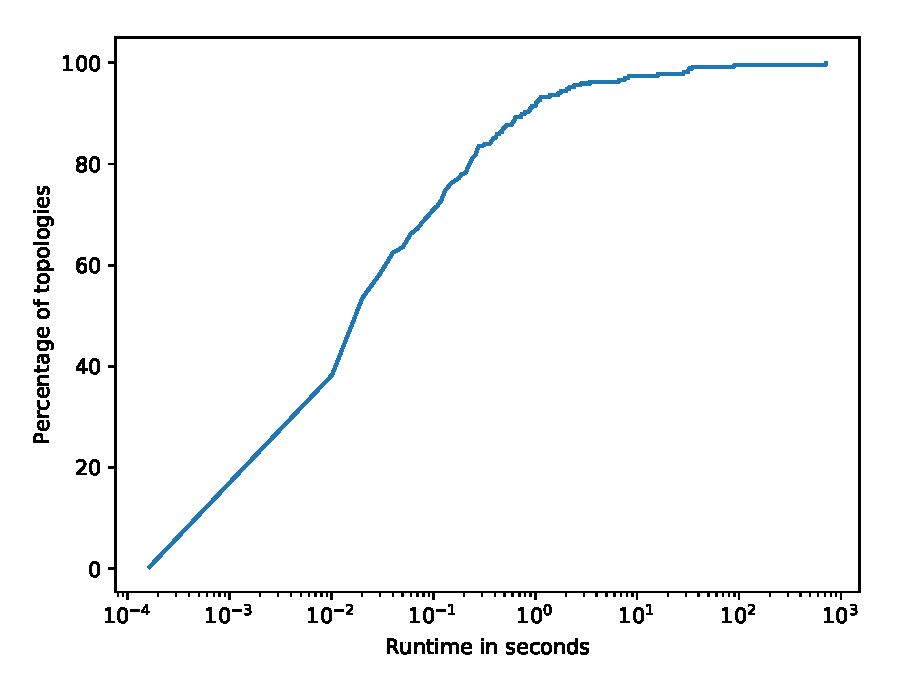
\includegraphics[width=.85\columnwidth]{./Network-lib/data/plot/minSegCover_runtime.eps}
\end{center}
\caption{Runtime CDF of Algorithm \ref{algo:min-seg-cover2} over all topologies.}
\label{fig:min-seg-cover-runtime}
\end{figure}

Figure \ref{fig:min-seg-cover-runtime-size} shows the runtime of ref{algo:min-seg-cover2} with respect to
the size of the topology $|G|$. We can observe that it indeed performs much better in practice than its theoretical
time complexity.

\begin{figure}
\begin{center}
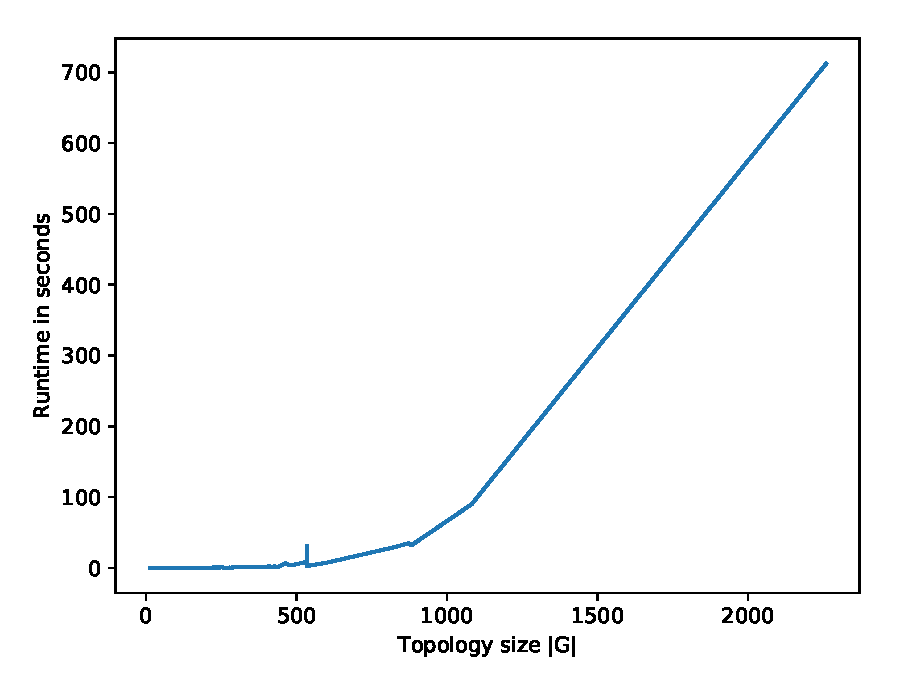
\includegraphics[width=.85\columnwidth]{./Network-lib/data/plot/minSegCover_runtime_by_size.eps}
\end{center}
\caption{Runtime by topology size of Algorithm \ref{algo:min-seg-cover2} over all topologies.}
\label{fig:min-seg-cover-runtime-size}
\end{figure}

Next, we analyze the segment cost of the sr-cycle covers produced by the algorithm. This gives a lower bound
on the segment cost of \emph{any} cycle cover on the given topologies. This is an important result as it shows
whether or not we can expect to be able to implement such a monitoring scheme on a segment routed network. As
we can see on Figure \ref{fig:min-seg-cover-segcost}, for more than $70\%$ we can find a cycle cover needing
at most a segment cost of $5$. This means that in most topologies such a sr-cycle cover is implementable even
on a network operating low end routers. Almost all topologies require a segment cost of at most $10$ showing
that network monitoring with segment routing is realistic for most topologies with high end routers. We wanted
to analyze the relationship between the size of the topology and the segment cost required for the sr-cycle cover.
The is shown in Figure \ref{fig:min-seg-cover-segcost-size}. We can see that the size does not seem to be 
correlated with the minimum segment cost.

\begin{figure}
\begin{center}
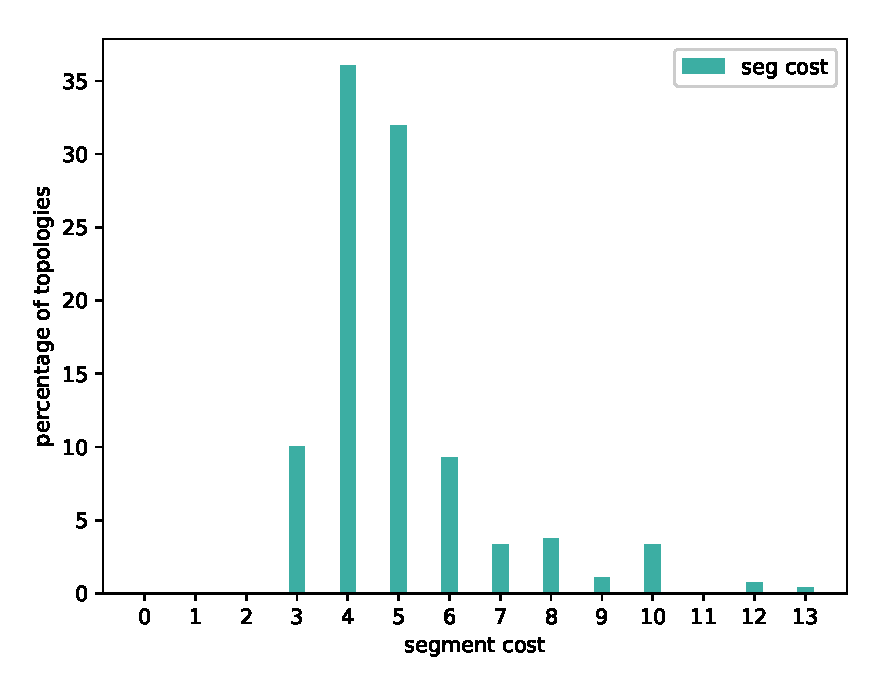
\includegraphics[width=.85\columnwidth]{./Network-lib/data/plot/minSegCover_segcost.eps}
\end{center}
\caption{Percentage of topologies for each segment cost.}
\label{fig:min-seg-cover-segcost}
\end{figure}


\begin{figure}
\begin{center}
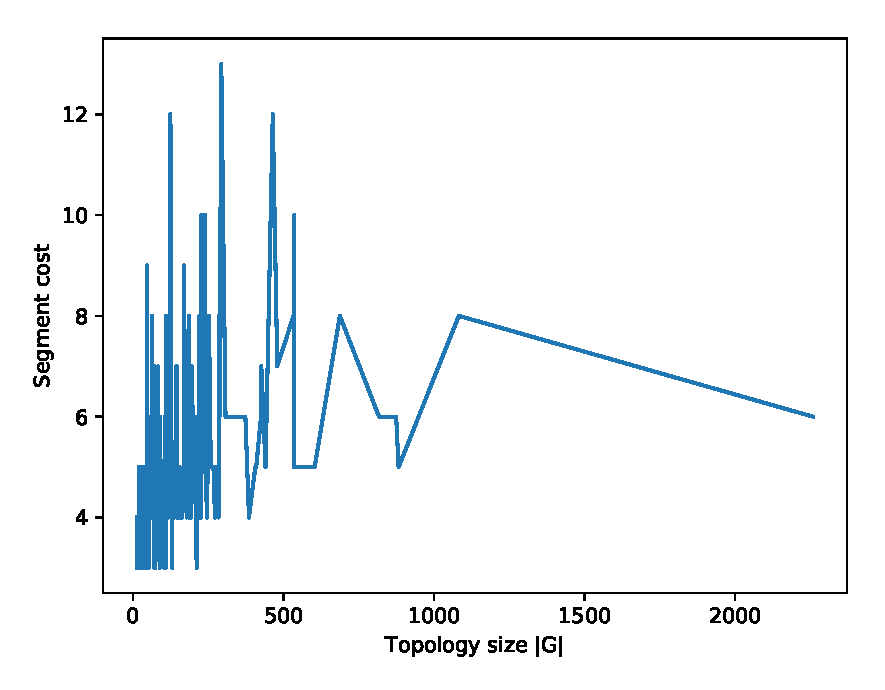
\includegraphics[width=.85\columnwidth]{./Network-lib/data/plot/minSegCover_segcost_by_size.eps}
\end{center}
\caption{Segment cost by topology size over all topologies.}
\label{fig:min-seg-cover-segcost-size}
\end{figure}


\section{Column generation cycle cover algorithm}

We saw in Chapter \ref{chapter:te} that column generation seemed to be a good framework to solve segment routing
problems. In this section we propose a column generation algorithm for computing lower bounds on the number of sr-cycles in a
minimum sr-cycle cover of a network. We also show how to derive from it an heuristic algorithm for Problem \ref{prob:min-cycle-cover}.

It is straightforward to express a MIP formulation for Problem \ref{prob:min-cycle-cover}. We define binary
variables $x_{\sr{c}}$ such that $x_{\sr{c}} = 1$ if and only if $\sr{c}$ is used in the cover. These variables
will be defined for every $\sr{c} \in \mathcal{C}^k_s$ where $k$ and $s$ are given as input. 

In terms of objective function, since we want to minimize the number of cycles in the cover, we can achieve this
by minimizing $\sum_{\sr{c} \in \mathcal{C}^k_s} x_{\sr{c}}$. This is so because this sum counts how many cycles
are used in the solution. For the constraints it is quite simple as well. We simply need to ensure that for each
edge $e \in E(G)$, there is at least one sr-cycle covering it, that is, there is at least one $\sr{c}$ such that
$x_{\sr{c}} = 1$ and $e \in E(\sr{c})$. We define the following identify function to simplify the expression of this constraints.

\begin{definition}
Given a network $G$ we define a function $I : \mathcal{P} \times E(G) \rightarrow \{0, 1\}$ such that
$I(\sr{p}, e) = 1$ if and only if $e \in E(\sr{p})$.
\end{definition}

\begin{center}
\begin{tabular}{crcllr}
\multicolumn{5}{l}{$\ccPrimalMip(G, k, s)$} \\[0.5cm] 
$\mathbf{min}$ & $\displaystyle \sum_{\sr{c} \in \mathcal{C}^k_s} x_{\sr{c}}$ & & & & \\[0.5cm]
$\textbf{s.t.}$ & $\displaystyle \sum_{\sr{c} \in \mathcal{C}^k_s} I(\sr{c}, e) \cdot x_{\sr{c}}$  & $\geq$ & $1$ & $\forall e \in E(G)$ & \\[0.5cm]
                & $x_{\sr{c}}$ & $\in$ & $\{0, 1\}$ & $\forall \sr{c} \in \mathcal{C}^k_s$
\end{tabular}
\end{center}

\subsection{Column generation}

We follow the same process that we did in Chapter \ref{chapter:te} to develop the column generation algorithm
for the minimum sr-cycle cover problem. Recall that CG is a technique for solving a LP and we have a MIP.
The first step is then to consider the LP-relaxation of $\ccPrimalMip$ and compute its dual.

\begin{center}
\begin{tabular}{crcllr}
\multicolumn{5}{l}{$\ccPrimalLp(G, k, s)$} \\[0.5cm] 
$\mathbf{min}$ & $\displaystyle \sum_{\sr{c} \in \mathcal{C}^k_s} x_{\sr{c}}$ & & & & \\[0.5cm]
$\textbf{s.t.}$ & $\displaystyle \sum_{\sr{c} \in \mathcal{C}^k_s} I(\sr{c}, e) \cdot x_{\sr{c}}$   & $\geq$ & $1$ & $\forall e \in E(G)$ & (P1) \\[0.5cm]
                & $x_{\sr{c}}$ & $\geq$  & $0$ & $\forall \sr{c} \in \mathcal{C}^k_s$
\end{tabular}
\end{center}

As before, the most natural relaxation would be to set $x_{\sr{c}} \in [0, 1]$ but our objective function guarantees that
this is equivalent to $x_{\sr{c}} \geq 0$. We chose the second one because it is equivalent and easier to work with.
The dual is obtained by following the same systematic procedure as before. By doing so we get the following LP.

\begin{center}
\begin{tabular}{crcllr}
\multicolumn{5}{l}{$\ccDualLp(G, k, s)$} \\[0.5cm] 
$\mathbf{max}$ & $\displaystyle \sum_{e \in E(G)} y_{e}$ & & & & \\[0.5cm]
$\textbf{s.t.}$ & $\displaystyle \sum_{e \in E(G)} I(\sr{c}, e) \cdot y_e$   & $\leq$ & $1$ & $\forall \sr{c} \in \mathcal{C}^k_s$ & (D1) \\[0.5cm]
                & $y_e$ & $\geq$ & $0$ & $\forall e \in E(G)$
\end{tabular}
\end{center}

The idea to solve $\ccPrimalLp$ is again to start with a small but feasible subset of sr-cycles $C \subseteq \mathcal{C}^k_s$ and 
slowly grow it until we can prove optimality. We denote the problems restricted to $C$ by adding $C$ as an argument, that is, by
$\ccPrimalLp(G, k, s, C)$ and $\ccDualLp(G, k, s, C)$. To find a new element $\sr{c}$ to add to $C$ we need to, given an optimal
solution $y^*$ of $\ccDualLp(G, k, s, C)$, find a sr-cycle $\sr{c}$ such that

$$
\sum_{e \in E(G)} I(\sr{c}, e) \cdot y^*_e = \sum_{e \in E(\sr{c})} y^*_e > 1.
$$

Solving this directly is \NPhard~since it can be shown to be equivalent to the longest path problem. 
Instead of trying to solve this pricing problem directly, we are going to see that by slightly changing the LP formulation we can
obtain a polynomial time solvable pricing problem.

\begin{definition}
Given a network $G$ we define a function $K : \mathcal{P} \times E(G) \rightarrow \mathbb{N}$ such that
$K(\sr{p}, e)$ equals the number of times $e$ is traversed by $\sr{p}$. Formally, if $\sr{p} = \langle x_1, \ldots, x_l \rangle$
$$
K(\sr{p}, e) = \sum_{i = 2}^l I(\sp(x^2_i, x^1_{i - 1}), e) + \sum_{i = 1 : x_i = e}^l 1.
$$
\end{definition}

By replacing $I$ by $K$ in the above formulations we still get a model for Problem \ref{prob:min-cycle-cover} since, the new constraints
corresponding to $(P1)$ with $I$ replaced by $K$, will still be true if and only if every edge is covered by at least one cycle. With this change the formulations become:

\begin{center}
\begin{tabular}{crcllr}
\multicolumn{5}{l}{$\ccPrimalLpK(G, k, s)$} \\[0.5cm] 
$\mathbf{min}$ & $\displaystyle \sum_{\sr{c} \in \mathcal{C}^k_s} x_{\sr{c}}$ & & & & \\[0.5cm]
$\textbf{s.t.}$ & $\displaystyle \sum_{\sr{c} \in \mathcal{C}^k_s} K(\sr{c}, e) \cdot x_{\sr{c}}$   & $\geq$ & $1$ & $\forall e \in E(G)$ &  \\[0.5cm]
                & $x_{\sr{c}}$ & $\geq$  & $0$ & $\forall \sr{c} \in \mathcal{C}^k_s$
\end{tabular}
\end{center}

\begin{center}
\begin{tabular}{crcllr}
\multicolumn{5}{l}{$\ccDualLpK(G, k, s)$} \\[0.5cm] 
$\mathbf{max}$ & $\displaystyle \sum_{e \in E(G)} y_{e}$ & & & & \\[0.5cm]
$\textbf{s.t.}$ & $\displaystyle \sum_{e \in E(G)} K(\sr{c}, e) \cdot y_e$   & $\leq$ & $1$ & $\forall \sr{c} \in \mathcal{C}^k_s$ &  \\[0.5cm]
                & $y_e$ & $\geq$ & $0$ & $\forall e \in E(G)$
\end{tabular}
\end{center}

The pricing problem now becomes the following one.

\begin{problem}{SRCC pricing}
\label{prob:cc-pricing}
\textbf{Input:} A network $G$, $k \in \mathbb{N}$, a source node $s \in V(G)$ and values $y_e \geq 0$ for each $e \in E(G)$.

\textbf{Output:} A sr-cycle $\sr{c} \in \mathcal{C}^k_s$ such that
$$
\sum_{e \in E(G)} K(\sr{c}, e) \cdot y_e > 1
$$
or report that no such sr-cycle exists.
\end{problem}

In order to solve Problem \ref{prob:cc-pricing}, we define a sr-metric $w$ such that 
$$
w(u, v) = \sum_{e \in \sp(u, v)} y_e
$$
and
$$
w(e) = y_e.
$$

With this metric, it is easy to see can see that
$$
w(\sr{c}) = \sum_{e \in E(G)} K(\sr{c}, e) \cdot y_e.
$$

Therefore we can solve the pricing problem by computing a sr-cycle $\sr{c}$ from $s$ to $s$ of segment
cost at most $k$ such that $w(\sr{c})$ is maximum. We have already shown in Chapter \ref{chapter:sr-optimal} that 
this problem can be solved in polynomial time. Therefore, we have the following theorem.

\begin{theorem}
Problem \ref{prob:cc-pricing} can be solved in polynomial time.
\end{theorem}

To start the column generation algorithm we need a feasible solution. In order to obtain one, we run Algorithm \ref{algo:min-seg-cover2} which also gives us
suitable source node $s$ and lower bound on the segment cost $k$. If the target segment cost is lower than $k$ then we immediately know
that a feasible solution does not exist. If it does, we use the cycles produced by the minimum segment cost cycle cover algorithm as an 
initial feasible solution for the column generation algorithm.

We evaluated the runtime of the column generation algorithm over all topologies. Figure \ref{fig:cc_runtime} shows a CDF of these runtimes.
The slowest topology took about $3$ hours so solve. Most topologies are solved in a very short amount of time and $98\%$ of the topologies
are solved in under $25$ minutes. These values are very reasonable given that the probing cycle only needs to be computed when the topology changes.

\begin{figure}
\begin{center}
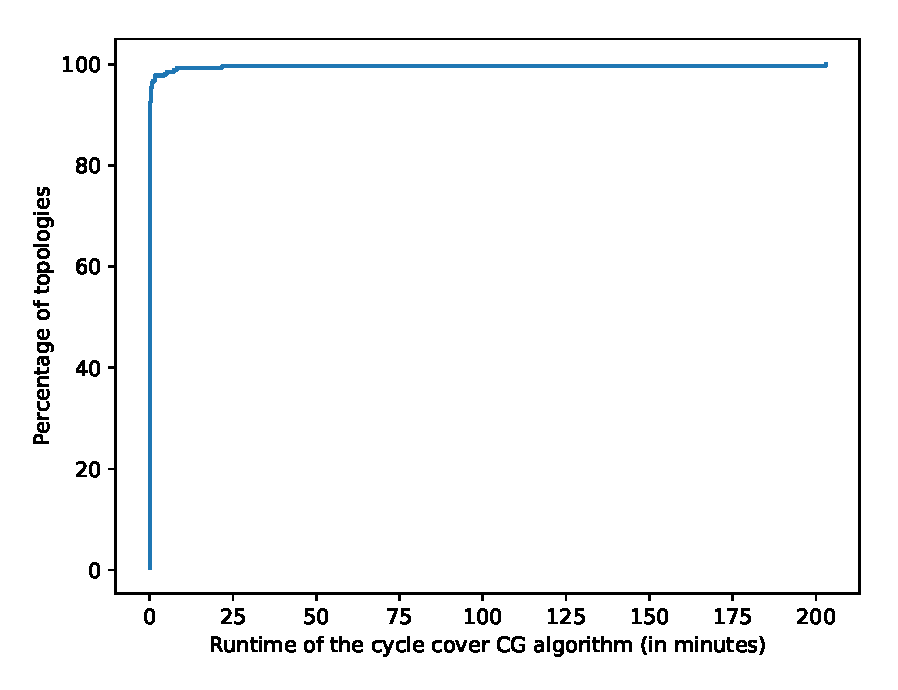
\includegraphics[width=.9\columnwidth]{./Network-lib/data/plot/minCycleCover_runtime_cdf.eps}
\end{center}
\caption{CDF of the runtime of the column generation cycle cover algorithm.}
\label{fig:cc_runtime}
\end{figure}

In the next section we will evaluate the lower bound provided by the column generation algorithm.


\subsection{Greedy algorithm}

We designed above a column generation algorithm for solving the LP relaxation of Problem \ref{prob:min-cycle-cover}. In this relaxation, an edge
can be covered fractionally by two sr-cycles or more. In this section we propose a greedy algorithm for converting these fractional solutions to proper 
solutions of Problem \ref{prob:min-cycle-cover}.

Let $C$ be the final set of sr-cycles. Our algorithm simply consists of selecting elements of $C$ 
while keeping track of the edges that are already covered until all of them are. At each step,
the sr-cycle that we selected is the sr-cycle that covers the maximum remaining uncovered edges. 

\begin{algorithm}[t]
\small
\caption{$\textsf{greedy-cc}\left( G, C \right)$}
\begin{algorithmic}[1]
%\algrule
\STATE $covered \gets \emptyset$
\STATE $cover \gets \emptyset$
\WHILE{$|U| < |E(G)|$}
  \STATE $\sr{c} \gets \sr{c} \in C \textbf{ such that } |E(\sr{c}) \cup covered| \textbf{ is maximum}$
  \STATE $cover \gets cover \cup \{ \sr{c} \}$
  \STATE $covered \gets covered \cup E(\sr{c})$
\ENDWHILE
\RETURN $cover$
\end{algorithmic}
\label{algo:greedy-cc}
\end{algorithm}

It is a well know result that this yields a logarithmic factor approximation. We prove this in the next theorem
for completeness.

\begin{theorem}
The set of cycles, $cover$, produced by Algorithm \ref{algo:greedy-cc} is such that
$$
opt_C \leq |cover| \leq \log|E(G)| \cdot opt_C
$$
where $opt_C$ is the size of a minimum over using only cycles from $C$.
\end{theorem}

\begin{proof}
Clearly, $opt_C \leq |cover|$. Let $m = |E(G)|$. 
Since the optimal solution relative to $C$ uses $opt_C$ sr-cycles, there must be at least one of them that covers at
least a fraction $1 \slash opt_C$ of the edges. If they were all below this ratio, they could not cover all edges.
Since we select the sr-cycle that covers the most uncovered edges, the first sr-cycle will cover
at least $1 \slash opt_C$ edges. Hence, after the first iteration, there are at most $m (1 - 1 \slash opt_C)$ edges left to cover. In the same way,
there must be a set that covers at least $1 \slash opt_C$ of these $m (1 - 1 \slash opt_C)$ edges. Since we select the 
sr-cycle covering the most edges, after the second iteration there are at most $m(1 - \slash opt_C)^2$ edges left. By repeating this argument,
we see that after $k$ iterations there are at most $m (1 - 1 \slash opt_C)^k$ edges left. Therefore, after $k = opt_C \log m$ iterations,
there are
$$
m (1 - 1 \slash opt_C)^{opt_C \log m} = m (1 \slash e)^{\log m} = m \cdot \frac{1}{e^{\log m}} = \frac{m}{m} = 1
$$
edges left. Hence $|cover| \leq \log m \cdot opt_C$.
\end{proof}

Ideally we would want to be able to prove that
$$
opt \leq |cover| \leq \log|E(G)| \cdot opt
$$
where $opt$ is the optimal solution over \emph{all} sr-cycles $\mathcal{C}^k_s$ but unfortunately this is not true in general.
However, since the fractional solution obtained with the column generation is a lower bound on $opt$ we can still evaluate how far
this gets us from the $opt$ in practice. Figure \ref{fig:sizes_3} shows the sizes of the minimum segment cost covers, the LP lower bound
and the sizes of the greedy covers.

\begin{figure}
\begin{center}
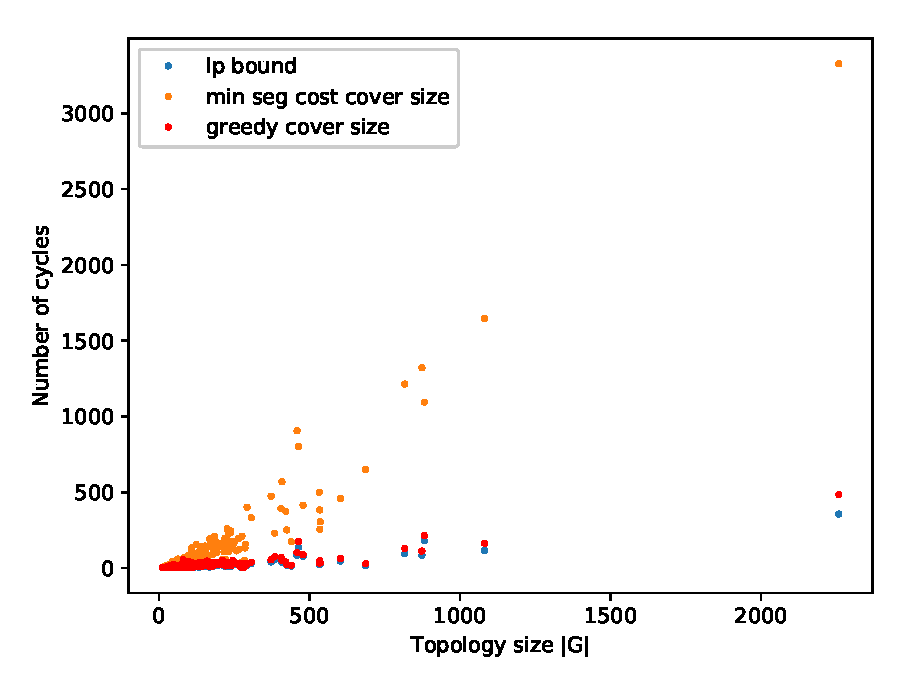
\includegraphics[width=.9\columnwidth]{./Network-lib/data/plot/minCycleCover_lowerbound.eps}
\end{center}
\caption{Lower bound, min seg cover size and greedy cover size shown by topologies size.}
\label{fig:sizes_3}
\end{figure}

We can see that the greedy solution is actually quite close to the lower bound and therefore it must also be
close to $opt$. To provide a better view of how close they are we computed a CDF of relative distance 
$$
\frac{greedy - lb}{lb}
$$
which is shown in Figure \ref{fig:cc_gap_cdf}. As a reference, with this metric, a value of $1$ 
means that the greedy solution uses twice the number of sr-cycle compared to the lower bound. 
We can see from the CDF that for $90\%$ of the instances we have an increase of at most
$50\%$ on the number of sr-cycles. Recall that this lower bound is not the actual number of sr-cycles in the optimal solution
but only an estimate. This means that our solution is actually even closer to the optimal solution.

\begin{figure}
\begin{center}
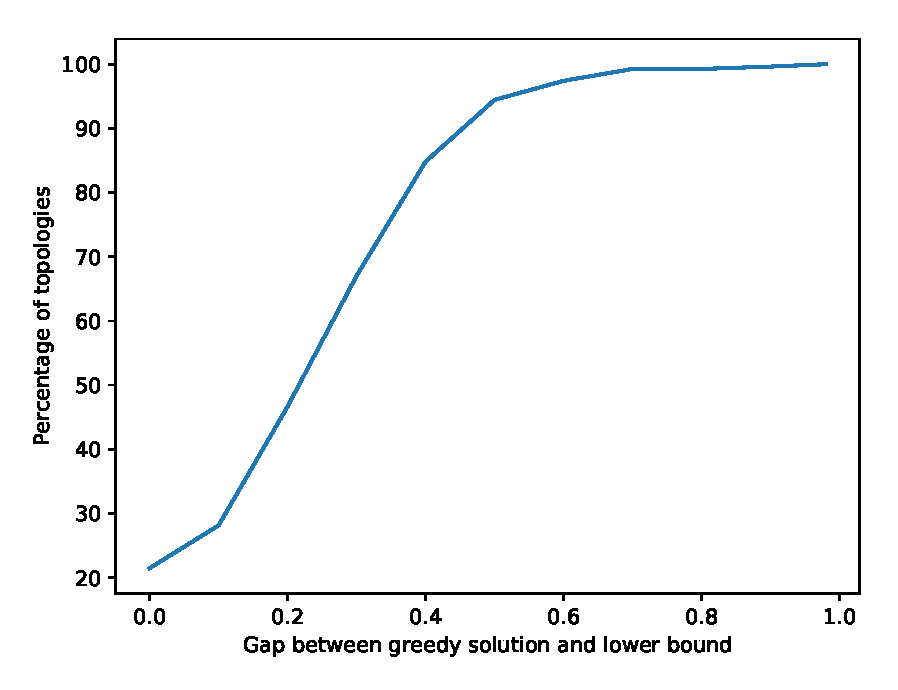
\includegraphics[width=.9\columnwidth]{./Network-lib/data/plot/minCycleCover_gapcdf.eps}
\end{center}
\caption{CDF of the gap between the greedy solution and the LP lower bound.}
\label{fig:cc_gap_cdf}
\end{figure}

The most important aspect is that by combining the minimum segment cost sr-cycle covers
with the column generation and the greedy algorithm we are able to greatly reduce the number of sr-cycles
in the minimum segment cost cover. Therefore, our solution is able to find sr-cycle covers that 
not only use the minimum amount of segments required for \emph{any} sr-cycle cover but also
are quite close to the minimum theoretical number of sr-cycles.


\section{Pinpointing single-link failures}

In this section we explain how to use a sr-cycle cover to detect single-link failures.

As mentioned in the introduction of this chapter, the idea is to have node $s$ 
regularly send monitoring probes over the sr-cycles of in a sr-cycle cover $C \subseteq \Csk$. Since we are using sr-cycles,
if the network is operating without failures, each probe must eventually come back to the vantage point $s$.
If at least one such probe does not come back, we know that at least one of the edges in the cycle associated with it
has a failure. We refer to the sr-cycles in the cycle cover $C$ as \emph{probing cycles}.

Let $\sr{c}$ be a cycle with a failure, that is, whose probe did not return. 
Because we use deterministic cycles, if we map $\sr{c}$ back to $G$, we get a cycle $c = (e_1, e_2, \ldots, e_l)$.
Recall that in this chapter we assume that the network $G$ is symmetric so that for each edge $e$ there is a reverse edge $\rev(e)$ and that
$\igp$ is symmetric if $\igp(e) = \rev(\igp(e))$.
The idea to detect the failure is to perform a binary search to find the largest $i$ such that
the cycle $c_i = (e_1, \ldots, e_i, \rev(e_i), \ldots, \rev(e_1))$ contains no failure. For each $i$ we send another 
probe over $c_i$ and check whether it comes back. If it does, then we know that the index we seek is greater than or equal to $i$. 
If it does not then the index must be strictly smaller than $i$. The single-link failure assumption is important for this process to work.
Because the probe did not cycle back, we know that one of 
$e_1, \ldots, e_l$ is faulty. Therefore, since we assume single-link
failure, we know that each reverse edge is not faulty. Hence, when we send a binary search probe on $c_i$, if it does not come back,
we know that the problem is in one of $e_1, \ldots, e_i$. We refer to these sr-cycles as \emph{identification cycles}.

Figure \ref{fig:bs-srcycle_new} illustrates this on an example with $l = 8$ and the failure is on edge $e_5$. We start the search with $i = 4$. The green dotted path
illustrates that the probe successfully returned to $v_1$. Thus we know that edges $e_1, e_2$ and $e_3$ are up.
The search will select $i = 6$ and this time the probe did not return. We conclude that the error is either in $e_4$ or $e_5$.
Finally, we send a probe on $c_5$ which returns. We finally conclude that the problem is on link $e_5$.

\begin{figure}
\begin{center}
\begin{tabular}{cc}
\begin{tikzpicture}[scale=0.75]
\node[scale=0.15] (a) at (3.000, 0.000) {\router{$v_1$}{router}};
\node[scale=0.15] (b) at (2.121, 2.121) {\router{$v_2$}{router}};
\node[scale=0.15] (c) at (0.000, 3.000) {\router{$v_3$}{router}};
\node[scale=0.15] (d) at (-2.121, 2.121) {\router{$v_4$}{router}};
\node[scale=0.15] (e) at (-3.000, 0.000) {\router{$v_5$}{router}};
\node[scale=0.15] (f) at (-2.121, -2.121) {\router{$v_6$}{router}};
\node[scale=0.15] (g) at (-0.000, -3.000) {\router{$v_7$}{router}};
\node[scale=0.15] (h) at (2.121, -2.121) {\router{$v_8$}{router}};

\draw[line width=2] (a) edge[above, sloped, bend right, ->] node[black,font=\bfseries] {\footnotesize \texttt{$e_1$}} (b);
\draw[line width=2] (b) edge[above, sloped, bend right, ->] node[black,font=\bfseries] {\footnotesize \texttt{$e_2$}} (c);
\draw[line width=2] (c) edge[above, sloped, bend right, ->] node[black,font=\bfseries] {\footnotesize \texttt{$e_3$}} (d);
\draw[line width=2] (d) edge[above, sloped, bend right, ->] node[black,font=\bfseries] {\footnotesize \texttt{$e_4$}} (e);
\draw[line width=2] (e) edge[below, sloped, bend right, ->] node[black,font=\bfseries] {\footnotesize \texttt{$e_5$}} (f);
\draw[line width=2] (f) edge[below, sloped, bend right, ->] node[black,font=\bfseries] {\footnotesize \texttt{$e_6$}} (g);
\draw[line width=2] (g) edge[below, sloped, bend right, ->] node[black,font=\bfseries] {\footnotesize \texttt{$e_7$}} (h);
\draw[line width=2] (h) edge[below, sloped, bend right, ->] node[black,font=\bfseries] {\footnotesize \texttt{$e_8$}} (a);
\draw (e) edge[sloped, bend right, ->] node[red, font=\bfseries] {\footnotesize \texttt{\Large \textsf{X}}} (f);

\draw[line width=2, gray] (a) edge[below, sloped, bend left, <-] node[gray,font=\bfseries] {\footnotesize \texttt{$\rev(e_1)$}} (b);
\draw[line width=2, gray] (b) edge[below, sloped, bend left, <-] node[gray,font=\bfseries] {\footnotesize \texttt{$\rev(e_2)$}} (c);
\draw[line width=2, gray] (c) edge[below, sloped, bend left, <-] node[gray,font=\bfseries] {\footnotesize \texttt{$\rev(e_3)$}} (d);
\draw[line width=2, gray] (d) edge[below, sloped, bend left, <-] node[gray,font=\bfseries] {\footnotesize \texttt{$\rev(e_4)$}} (e);
\draw[line width=2, gray] (e) edge[above, sloped, bend left, <-] node[gray,font=\bfseries] {\footnotesize \texttt{$\rev(e_5)$}} (f);

\draw[line width=2, gray] (f) edge[above, sloped, bend left, <-] node[gray,font=\bfseries] {\footnotesize \texttt{$\rev(e_6)$}} (g);
\draw[line width=2, gray] (g) edge[above, sloped, bend left, <-] node[gray,font=\bfseries] {\footnotesize \texttt{$\rev(e_7)$}} (h);
\draw[line width=2, gray] (h) edge[above, sloped, bend left, <-] node[gray,font=\bfseries] {\footnotesize \texttt{$\rev(e_8)$}} (a);

\draw[darkgreen, ultra thick, dotted, ->] plot [smooth] coordinates { ($(a)+(0.5,0)$) ($(b)+(0,0.5)$) ($(c)+(0,0.5)$) ($(d)+(0,0.5)$) ($(d)+(-0.5,0)$) ($(d)+(0,-0.5)$) ($(c)+(0,-0.5)$) ($(b)+(0,-0.5)$) ($(a)$) };

\end{tikzpicture}

&

\begin{tikzpicture}[scale=0.75]
\node[scale=0.15] (1) at (3.000, 0.000) {\router{$v_1$}{router}};
\node[scale=0.15] (2) at (2.121, 2.121) {\router{$v_2$}{router}};
\node[scale=0.15] (3) at (0.000, 3.000) {\router{$v_3$}{router}};
\node[scale=0.15] (4) at (-2.121, 2.121) {\router{$v_4$}{green}};
\node[scale=0.15] (5) at (-3.000, 0.000) {\router{$v_5$}{router}};
\node[scale=0.15] (6) at (-2.121, -2.121) {\router{$v_6$}{router}};
\node[scale=0.15] (7) at (-0.000, -3.000) {\router{$v_7$}{router}};
\node[scale=0.15] (8) at (2.121, -2.121) {\router{$v_8$}{router}};

\draw[line width=2, darkgreen] (1) edge[above, sloped, bend right, ->] node[black,font=\bfseries] {\footnotesize \texttt{$e_1$}} (2);
\draw[line width=2, darkgreen] (2) edge[above, sloped, bend right, ->] node[black,font=\bfseries] {\footnotesize \texttt{$e_2$}} (3);
\draw[line width=2, darkgreen] (3) edge[above, sloped, bend right, ->] node[black,font=\bfseries] {\footnotesize \texttt{$e_3$}} (4);
\draw[line width=2] (4) edge[above, sloped, bend right, ->] node[black,font=\bfseries] {\footnotesize \texttt{$e_4$}} (5);
\draw[line width=2] (5) edge[below, sloped, bend right, ->] node[black,font=\bfseries] {\footnotesize \texttt{$e_5$}} (6);
\draw[line width=2] (6) edge[below, sloped, bend right, ->] node[black,font=\bfseries] {\footnotesize \texttt{$e_6$}} (7);
\draw[line width=2] (7) edge[below, sloped, bend right, ->] node[black,font=\bfseries] {\footnotesize \texttt{$e_7$}} (8);
\draw[line width=2] (8) edge[below, sloped, bend right, ->] node[black,font=\bfseries] {\footnotesize \texttt{$e_8$}} (1);
\draw (5) edge[sloped, bend right, ->] node[red, font=\bfseries] {\footnotesize \texttt{\Large \textsf{X}}} (6);

\draw[line width=2, gray, darkgreen] (1) edge[below, sloped, bend left, <-] node[gray,font=\bfseries] {\footnotesize \texttt{$\rev(e_1)$}} (2);
\draw[line width=2, gray, darkgreen] (2) edge[below, sloped, bend left, <-] node[gray,font=\bfseries] {\footnotesize \texttt{$\rev(e_2)$}} (3);
\draw[line width=2, gray, darkgreen] (3) edge[below, sloped, bend left, <-] node[gray,font=\bfseries] {\footnotesize \texttt{$\rev(e_3)$}} (4);
\draw[line width=2, gray] (4) edge[below, sloped, bend left, <-] node[gray,font=\bfseries] {\footnotesize \texttt{$\rev(e_4)$}} (5);
\draw[line width=2, gray] (5) edge[above, sloped, bend left, <-] node[gray,font=\bfseries] {\footnotesize \texttt{$\rev(e_5)$}} (6);
\draw[line width=2, gray] (6) edge[above, sloped, bend left, <-] node[gray,font=\bfseries] {\footnotesize \texttt{$\rev(e_6)$}} (7);
\draw[line width=2, gray] (7) edge[above, sloped, bend left, <-] node[gray,font=\bfseries] {\footnotesize \texttt{$\rev(e_7)$}} (8);
\draw[line width=2, gray] (8) edge[above, sloped, bend left, <-] node[gray,font=\bfseries] {\footnotesize \texttt{$\rev(e_8)$}} (1);

\draw[red!50!black, ultra thick, dotted, ->] plot [smooth] coordinates { 
($(a)+(0.5,0)$) ($(b)+(0,0.5)$) ($(c)+(0,0.5)$) ($(d)+(0,0.5)$) ($(e)+(-0.5,0)$) ($(f)+(-0.5,0)$) 
($(f)+(0,-0.5)$) ($(f)+(0.5,0)$) ($(e)+(0.5,0)$) ($(d)+(0,-0.5)$) ($(c)+(0,-0.5)$) ($(b)+(0,-0.5)$) ($(a)$) 
};

\end{tikzpicture}

\\

\footnotesize

First step of binary search. Success.

&

\footnotesize

Second step of binary search. Failure.

\\

\footnotesize

Edges $e_1, e_2, e_3$ are up.

&

\footnotesize

One of $e_4, e_5$ is down.

\\[0.5cm]

\begin{tikzpicture}[scale=0.75]
\node[scale=0.15] (1) at (3.000, 0.000) {\router{$v_1$}{router}};
\node[scale=0.15] (2) at (2.121, 2.121) {\router{$v_2$}{router}};
\node[scale=0.15] (3) at (0.000, 3.000) {\router{$v_3$}{router}};
\node[scale=0.15] (4) at (-2.121, 2.121) {\router{$v_4$}{green}};
\node[scale=0.15] (5) at (-3.000, 0.000) {\router{$v_5$}{router}};
\node[scale=0.15] (6) at (-2.121, -2.121) {\router{$v_6$}{red!50!white}};
\node[scale=0.15] (7) at (-0.000, -3.000) {\router{$v_7$}{router}};
\node[scale=0.15] (8) at (2.121, -2.121) {\router{$v_8$}{router}};

\draw[line width=2, darkgreen] (1) edge[above, sloped, bend right, ->] node[black,font=\bfseries] {\footnotesize \texttt{$e_1$}} (2);
\draw[line width=2, darkgreen] (2) edge[above, sloped, bend right, ->] node[black,font=\bfseries] {\footnotesize \texttt{$e_2$}} (3);
\draw[line width=2, darkgreen] (3) edge[above, sloped, bend right, ->] node[black,font=\bfseries] {\footnotesize \texttt{$e_3$}} (4);
\draw[line width=2] (4) edge[above, sloped, bend right, ->] node[black,font=\bfseries] {\footnotesize \texttt{$e_4$}} (5);
\draw[line width=2] (5) edge[below, sloped, bend right, ->] node[black,font=\bfseries] {\footnotesize \texttt{$e_5$}} (6);
\draw[line width=2] (6) edge[below, sloped, bend right, ->] node[black,font=\bfseries] {\footnotesize \texttt{$e_6$}} (7);
\draw[line width=2] (7) edge[below, sloped, bend right, ->] node[black,font=\bfseries] {\footnotesize \texttt{$e_7$}} (8);
\draw[line width=2] (8) edge[below, sloped, bend right, ->] node[black,font=\bfseries] {\footnotesize \texttt{$e_8$}} (1);
\draw (5) edge[sloped, bend right, ->] node[red, font=\bfseries] {\footnotesize \texttt{\Large \textsf{X}}} (6);

\draw[line width=2, gray, darkgreen] (1) edge[below, sloped, bend left, <-] node[gray,font=\bfseries] {\footnotesize \texttt{$\rev(e_1)$}} (2);
\draw[line width=2, gray, darkgreen] (2) edge[below, sloped, bend left, <-] node[gray,font=\bfseries] {\footnotesize \texttt{$\rev(e_2)$}} (3);
\draw[line width=2, gray, darkgreen] (3) edge[below, sloped, bend left, <-] node[gray,font=\bfseries] {\footnotesize \texttt{$\rev(e_3)$}} (4);
\draw[line width=2, gray] (4) edge[below, sloped, bend left, <-] node[gray,font=\bfseries] {\footnotesize \texttt{$\rev(e_4)$}} (5);
\draw[line width=2, gray] (5) edge[above, sloped, bend left, <-] node[gray,font=\bfseries] {\footnotesize \texttt{$\rev(e_5)$}} (6);
\draw[line width=2, gray] (6) edge[above, sloped, bend left, <-] node[gray,font=\bfseries] {\footnotesize \texttt{$\rev(e_6)$}} (7);
\draw[line width=2, gray] (7) edge[above, sloped, bend left, <-] node[gray,font=\bfseries] {\footnotesize \texttt{$\rev(e_7)$}} (8);
\draw[line width=2, gray] (8) edge[above, sloped, bend left, <-] node[gray,font=\bfseries] {\footnotesize \texttt{$\rev(e_8)$}} (1);

\draw[darkgreen, ultra thick, dotted, ->] plot [smooth] coordinates { 
($(a)+(0.5,0)$) ($(b)+(0,0.5)$) ($(c)+(0,0.5)$) ($(d)+(0,0.5)$) ($(e)+(-0.5,0)$) 
($(e)+(0,-0.5)$) ($(e)+(0.5,0)$) ($(d)+(0,-0.5)$) ($(c)+(0,-0.5)$) ($(b)+(0,-0.5)$) ($(a)$) 
};

\end{tikzpicture}

&


\begin{tikzpicture}[scale=0.75]
\node[scale=0.15] (1) at (3.000, 0.000) {\router{$v_1$}{router}};
\node[scale=0.15] (2) at (2.121, 2.121) {\router{$v_2$}{router}};
\node[scale=0.15] (3) at (0.000, 3.000) {\router{$v_3$}{router}};
\node[scale=0.15] (4) at (-2.121, 2.121) {\router{$v_4$}{green}};
\node[scale=0.15] (5) at (-3.000, 0.000) {\router{$v_5$}{green}};
\node[scale=0.15] (6) at (-2.121, -2.121) {\router{$v_6$}{red!50!white}};
\node[scale=0.15] (7) at (-0.000, -3.000) {\router{$v_7$}{router}};
\node[scale=0.15] (8) at (2.121, -2.121) {\router{$v_8$}{router}};

\draw[line width=2, darkgreen] (1) edge[above, sloped, bend right, ->] node[black,font=\bfseries] {\footnotesize \texttt{$e_1$}} (2);
\draw[line width=2, darkgreen] (2) edge[above, sloped, bend right, ->] node[black,font=\bfseries] {\footnotesize \texttt{$e_2$}} (3);
\draw[line width=2, darkgreen] (3) edge[above, sloped, bend right, ->] node[black,font=\bfseries] {\footnotesize \texttt{$e_3$}} (4);
\draw[line width=2, darkgreen] (4) edge[above, sloped, bend right, ->] node[black,font=\bfseries] {\footnotesize \texttt{$e_4$}} (5);
\draw[line width=2] (5) edge[below, red!50!black, sloped, bend right, ->] node[black,font=\bfseries] {\footnotesize \texttt{$e_5$}} (6);
\draw[line width=2, opacity=0] (5) edge[red!50!black, sloped, bend right, ->] node (e5) {} (6);
\draw (5) edge[sloped, bend right, ->] node[red, font=\bfseries] {\footnotesize \texttt{\Large \textsf{X}}} (6);

\draw[line width=2] (6) edge[below, sloped, bend right, ->] node[black,font=\bfseries] {\footnotesize \texttt{$e_6$}} (7);
\draw[line width=2] (7) edge[below, sloped, bend right, ->] node[black,font=\bfseries] {\footnotesize \texttt{$e_7$}} (8);
\draw[line width=2] (8) edge[below, sloped, bend right, ->] node[black,font=\bfseries] {\footnotesize \texttt{$e_8$}} (1);

\draw[line width=2, gray, darkgreen] (1) edge[below, sloped, bend left, <-] node[gray,font=\bfseries] {\footnotesize \texttt{$\rev(e_1)$}} (2);
\draw[line width=2, gray, darkgreen] (2) edge[below, sloped, bend left, <-] node[gray,font=\bfseries] {\footnotesize \texttt{$\rev(e_2)$}} (3);
\draw[line width=2, gray, darkgreen] (3) edge[below, sloped, bend left, <-] node[gray,font=\bfseries] {\footnotesize \texttt{$\rev(e_3)$}} (4);
\draw[line width=2, gray, darkgreen] (4) edge[below, sloped, bend left, <-] node[gray,font=\bfseries] {\footnotesize \texttt{$\rev(e_4)$}} (5);
\draw[line width=2, gray, gray] (5) edge[above, sloped, bend left, <-] node[gray,font=\bfseries] {\footnotesize \texttt{$\rev(e_5)$}} (6);
%\draw[line width=2, gray, red!50!black, opacity=0] (5) edge[sloped, bend left, <-] node[gray,font=\bfseries] (re5) {} (6);


\draw[line width=2, gray] (6) edge[above, sloped, bend left, <-] node[gray,font=\bfseries] {\footnotesize \texttt{$\rev(e_6)$}} (7);
\draw[line width=2, gray] (7) edge[above, sloped, bend left, <-] node[gray,font=\bfseries] {\footnotesize \texttt{$\rev(e_7)$}} (8);
\draw[line width=2, gray] (8) edge[above, sloped, bend left, <-] node[gray,font=\bfseries] {\footnotesize \texttt{$\rev(e_8)$}} (1);

%\draw[darkgreen, ultra thick, dotted, ->] plot [smooth] coordinates { 
%($(a)+(0.5,0)$) ($(b)+(0,0.5)$) ($(c)+(0,0.5)$) ($(d)+(0,0.5)$) ($(e)+(-0.5,0)$) 
%($(e)+(0,-0.5)$) ($(e)+(0.5,0)$) ($(d)+(0,-0.5)$) ($(c)+(0,-0.5)$) ($(b)+(0,-0.5)$) ($(a)$) 
%};

%\node (fail) at (0, 0) {failure};

%\draw[->, dashed] (fail) -- (e5);
%\draw[->, dashed] (fail) -- (re5);


\end{tikzpicture}

\\

\footnotesize

Third step of binary search. Success.

&

\footnotesize

End of the search.

\\

\footnotesize

Edges $e_4$ is up.

&

\footnotesize

Failure detected in $e_5$.

\end{tabular}
\end{center}
\caption{Binary search to identify the failure (single-link failure assumption).}
\label{fig:bs-srcycle_new}
\end{figure}

To illustrate why the single link-failure assumption is important, let's see happens with this process
when multiple failures occur. Imagine the same example as in Figure \ref{fig:bs-srcycle_new} but assume that
edge $\rev(e_3)$ is also down. In this case the first binary search probe will fail to return and the search
will stop at $i = 3$ and the algorithm will say that the problem is on edge $e_3$. However $e_3$ is up
and it is $\rev(e_3)$ that prevents the probe to return. This shows that with multiple failures, we cannot
know exactly which link is down. However, we still can say that either $e_3$ is down \emph{or} $\rev(e_3)$ is
down. Figure \ref{fig:bs-srcycle_new2} illustrates this.

This means that in presence of multiple link failures, we cannot tell exactly which link is down but we can
still find a set of two links $\{ e, \rev(e) \}$ such that we are sure that at least one of them is down.

\begin{figure}
\begin{center}
\begin{tabular}{cc}
\begin{tikzpicture}[scale=0.75]
\node[scale=0.15] (a) at (3.000, 0.000) {\router{$v_1$}{router}};
\node[scale=0.15] (b) at (2.121, 2.121) {\router{$v_2$}{router}};
\node[scale=0.15] (c) at (0.000, 3.000) {\router{$v_3$}{router}};
\node[scale=0.15] (d) at (-2.121, 2.121) {\router{$v_4$}{router}};
\node[scale=0.15] (e) at (-3.000, 0.000) {\router{$v_5$}{router}};
\node[scale=0.15] (f) at (-2.121, -2.121) {\router{$v_6$}{router}};
\node[scale=0.15] (g) at (-0.000, -3.000) {\router{$v_7$}{router}};
\node[scale=0.15] (h) at (2.121, -2.121) {\router{$v_8$}{router}};

\draw[line width=2] (a) edge[above, sloped, bend right, ->] node[black,font=\bfseries] {\footnotesize \texttt{$e_1$}} (b);
\draw[line width=2] (b) edge[above, sloped, bend right, ->] node[black,font=\bfseries] {\footnotesize \texttt{$e_2$}} (c);
\draw[line width=2] (c) edge[above, sloped, bend right, ->] node[black,font=\bfseries] {\footnotesize \texttt{$e_3$}} (d);
\draw[line width=2] (d) edge[above, sloped, bend right, ->] node[black,font=\bfseries] {\footnotesize \texttt{$e_4$}} (e);
\draw[line width=2] (e) edge[below, sloped, bend right, ->] node[black,font=\bfseries] {\footnotesize \texttt{$e_5$}} (f);
\draw[line width=2] (f) edge[below, sloped, bend right, ->] node[black,font=\bfseries] {\footnotesize \texttt{$e_6$}} (g);
\draw[line width=2] (g) edge[below, sloped, bend right, ->] node[black,font=\bfseries] {\footnotesize \texttt{$e_7$}} (h);
\draw[line width=2] (h) edge[below, sloped, bend right, ->] node[black,font=\bfseries] {\footnotesize \texttt{$e_8$}} (a);
\draw (e) edge[sloped, bend right, ->] node[red, font=\bfseries] {\Large \textsf{X}} (f);

\draw[line width=2, gray] (a) edge[below, sloped, bend left, <-] node[gray,font=\bfseries] {\footnotesize \texttt{$\rev(e_1)$}} (b);
\draw[line width=2, gray] (b) edge[below, sloped, bend left, <-] node[gray,font=\bfseries] {\footnotesize \texttt{$\rev(e_2)$}} (c);
\draw[line width=2, gray] (c) edge[below, sloped, bend left, <-] node[gray,font=\bfseries] {\footnotesize \texttt{$\rev(e_3)$}} (d);
\draw[line width=2, gray] (d) edge[below, sloped, bend left, <-] node[gray,font=\bfseries] {\footnotesize \texttt{$\rev(e_4)$}} (e);
\draw[line width=2, gray] (e) edge[above, sloped, bend left, <-] node[gray,font=\bfseries] {\footnotesize \texttt{$\rev(e_5)$}} (f);
\draw[line width=2, gray] (c) edge[sloped, bend left, <-] node[red,font=\bfseries] {\Large \textsf{X}} (d);

\draw[line width=2, gray] (f) edge[above, sloped, bend left, <-] node[gray,font=\bfseries] {\footnotesize \texttt{$\rev(e_6)$}} (g);
\draw[line width=2, gray] (g) edge[above, sloped, bend left, <-] node[gray,font=\bfseries] {\footnotesize \texttt{$\rev(e_7)$}} (h);
\draw[line width=2, gray] (h) edge[above, sloped, bend left, <-] node[gray,font=\bfseries] {\footnotesize \texttt{$\rev(e_8)$}} (a);

\draw[red!50!black, ultra thick, dotted, ->] plot [smooth] coordinates { ($(a)+(0.5,0)$) ($(b)+(0,0.5)$) ($(c)+(0,0.5)$) ($(d)+(0,0.5)$) ($(d)+(-0.5,0)$) ($(d)+(0,-0.5)$) ($(c)+(0,-0.5)$) ($(b)+(0,-0.5)$) ($(a)$) };

\end{tikzpicture}

&

\begin{tikzpicture}[scale=0.75]
\node[scale=0.15] (1) at (3.000, 0.000) {\router{$v_1$}{router}};
\node[scale=0.15] (2) at (2.121, 2.121) {\router{$v_2$}{router}};
\node[scale=0.15] (3) at (0.000, 3.000) {\router{$v_3$}{router}};
\node[scale=0.15] (4) at (-2.121, 2.121) {\router{$v_4$}{red!50!white}};
\node[scale=0.15] (5) at (-3.000, 0.000) {\router{$v_5$}{router}};
\node[scale=0.15] (6) at (-2.121, -2.121) {\router{$v_6$}{router}};
\node[scale=0.15] (7) at (-0.000, -3.000) {\router{$v_7$}{router}};
\node[scale=0.15] (8) at (2.121, -2.121) {\router{$v_8$}{router}};

\draw[line width=2] (1) edge[above, sloped, bend right, ->] node[black,font=\bfseries] {\footnotesize \texttt{$e_1$}} (2);
\draw[line width=2] (2) edge[above, sloped, bend right, ->] node[black,font=\bfseries] {\footnotesize \texttt{$e_2$}} (3);
\draw[line width=2] (3) edge[above, sloped, bend right, ->] node[black,font=\bfseries] {\footnotesize \texttt{$e_3$}} (4);
\draw[line width=2] (4) edge[above, sloped, bend right, ->] node[black,font=\bfseries] {\footnotesize \texttt{$e_4$}} (5);
\draw[line width=2] (5) edge[below, sloped, bend right, ->] node[black,font=\bfseries] {\footnotesize \texttt{$e_5$}} (6);
\draw[line width=2] (6) edge[below, sloped, bend right, ->] node[black,font=\bfseries] {\footnotesize \texttt{$e_6$}} (7);
\draw[line width=2] (7) edge[below, sloped, bend right, ->] node[black,font=\bfseries] {\footnotesize \texttt{$e_7$}} (8);
\draw[line width=2] (8) edge[below, sloped, bend right, ->] node[black,font=\bfseries] {\footnotesize \texttt{$e_8$}} (1);
\draw (5) edge[sloped, bend right, ->] node[red, font=\bfseries] {\footnotesize \texttt{\Large \textsf{X}}} (6);

\draw[line width=2, gray] (1) edge[below, sloped, bend left, <-] node[gray,font=\bfseries] {\footnotesize \texttt{$\rev(e_1)$}} (2);
\draw[line width=2, gray] (2) edge[below, sloped, bend left, <-] node[gray,font=\bfseries] {\footnotesize \texttt{$\rev(e_2)$}} (3);
\draw[line width=2, gray] (3) edge[below, sloped, bend left, <-] node[gray,font=\bfseries] {\footnotesize \texttt{$\rev(e_3)$}} (4);
\draw[line width=2, gray] (4) edge[below, sloped, bend left, <-] node[gray,font=\bfseries] {\footnotesize \texttt{$\rev(e_4)$}} (5);
\draw[line width=2, gray] (5) edge[above, sloped, bend left, <-] node[gray,font=\bfseries] {\footnotesize \texttt{$\rev(e_5)$}} (6);
\draw[line width=2, gray] (6) edge[above, sloped, bend left, <-] node[gray,font=\bfseries] {\footnotesize \texttt{$\rev(e_6)$}} (7);
\draw[line width=2, gray] (7) edge[above, sloped, bend left, <-] node[gray,font=\bfseries] {\footnotesize \texttt{$\rev(e_7)$}} (8);
\draw[line width=2, gray] (8) edge[above, sloped, bend left, <-] node[gray,font=\bfseries] {\footnotesize \texttt{$\rev(e_8)$}} (1);
\draw[line width=2, gray] (c) edge[sloped, bend left, <-] node[red,font=\bfseries] {\Large \textsf{X}} (d);

\draw[darkgreen, ultra thick, dotted, ->] plot [smooth] coordinates 
{ ($(a)+(0.5,0)$) ($(b)+(0.5,0.5)$) ($(b)+(0,0.5)$) ($(b)+(-0.5,0)$)($(a)$) };

\end{tikzpicture}

\\

\footnotesize

First step of binary search. Failure.

&

\footnotesize

Second step of binary search. Success.

\\

\footnotesize

One of $e_1, e_2, e_3, \rev(e_3), \rev(e_2), \rev(e_1)$ is down.

&

\footnotesize

Edges $e_1, \rev(e_1)$ are up.

\\[0.5cm]

\begin{tikzpicture}[scale=0.75]
\node[scale=0.15] (1) at (3.000, 0.000) {\router{$v_1$}{router}};
\node[scale=0.15] (2) at (2.121, 2.121) {\router{$v_2$}{green}};
\node[scale=0.15] (3) at (0.000, 3.000) {\router{$v_3$}{router}};
\node[scale=0.15] (4) at (-2.121, 2.121) {\router{$v_4$}{red!50!white}};
\node[scale=0.15] (5) at (-3.000, 0.000) {\router{$v_5$}{router}};
\node[scale=0.15] (6) at (-2.121, -2.121) {\router{$v_6$}{router}};
\node[scale=0.15] (7) at (-0.000, -3.000) {\router{$v_7$}{router}};
\node[scale=0.15] (8) at (2.121, -2.121) {\router{$v_8$}{router}};

\draw[line width=2] (1) edge[darkgreen, sloped, bend right, ->] node[black,font=\bfseries] {\footnotesize \texttt{$e_1$}} (2);
\draw[line width=2] (2) edge[above, sloped, bend right, ->] node[black,font=\bfseries] {\footnotesize \texttt{$e_2$}} (3);
\draw[line width=2] (3) edge[above, sloped, bend right, ->] node[black,font=\bfseries] {\footnotesize \texttt{$e_3$}} (4);
\draw[line width=2] (4) edge[above, sloped, bend right, ->] node[black,font=\bfseries] {\footnotesize \texttt{$e_4$}} (5);
\draw[line width=2] (5) edge[below, sloped, bend right, ->] node[black,font=\bfseries] {\footnotesize \texttt{$e_5$}} (6);
\draw[line width=2] (6) edge[below, sloped, bend right, ->] node[black,font=\bfseries] {\footnotesize \texttt{$e_6$}} (7);
\draw[line width=2] (7) edge[below, sloped, bend right, ->] node[black,font=\bfseries] {\footnotesize \texttt{$e_7$}} (8);
\draw[line width=2] (8) edge[below, sloped, bend right, ->] node[black,font=\bfseries] {\footnotesize \texttt{$e_8$}} (1);
\draw (5) edge[sloped, bend right, ->] node[red, font=\bfseries] {\footnotesize \texttt{\Large \textsf{X}}} (6);

\draw[line width=2, gray] (1) edge[darkgreen, below, sloped, bend left, <-] node[gray,font=\bfseries] {\footnotesize \texttt{$\rev(e_1)$}} (2);
\draw[line width=2, gray] (2) edge[below, sloped, bend left, <-] node[gray,font=\bfseries] {\footnotesize \texttt{$\rev(e_2)$}} (3);
\draw[line width=2, gray] (3) edge[below, sloped, bend left, <-] node[gray,font=\bfseries] {\footnotesize \texttt{$\rev(e_3)$}} (4);
\draw[line width=2, gray] (4) edge[below, sloped, bend left, <-] node[gray,font=\bfseries] {\footnotesize \texttt{$\rev(e_4)$}} (5);
\draw[line width=2, gray] (5) edge[above, sloped, bend left, <-] node[gray,font=\bfseries] {\footnotesize \texttt{$\rev(e_5)$}} (6);
\draw[line width=2, gray] (6) edge[above, sloped, bend left, <-] node[gray,font=\bfseries] {\footnotesize \texttt{$\rev(e_6)$}} (7);
\draw[line width=2, gray] (7) edge[above, sloped, bend left, <-] node[gray,font=\bfseries] {\footnotesize \texttt{$\rev(e_7)$}} (8);
\draw[line width=2, gray] (8) edge[above, sloped, bend left, <-] node[gray,font=\bfseries] {\footnotesize \texttt{$\rev(e_8)$}} (1);
\draw[line width=2, gray] (c) edge[sloped, bend left, <-] node[red,font=\bfseries] {\Large \textsf{X}} (d);

\draw[darkgreen, ultra thick, dotted, ->] plot [smooth] coordinates 
{ ($(a)+(0.5,0)$) ($(b)+(0,0.5)$) ($(c)+(0,0.5)$) ($(c)+(-0.5,0)$) ($(c)+(0,-0.5)$) ($(b)+(0,-0.5)$) ($(a)$) };

\end{tikzpicture}


&


\begin{tikzpicture}[scale=0.75]
\node[scale=0.15] (1) at (3.000, 0.000) {\router{$v_1$}{router}};
\node[scale=0.15] (2) at (2.121, 2.121) {\router{$v_2$}{green}};
\node[scale=0.15] (3) at (0.000, 3.000) {\router{$v_3$}{green}};
\node[scale=0.15] (4) at (-2.121, 2.121) {\router{$v_4$}{red!50!white}};
\node[scale=0.15] (5) at (-3.000, 0.000) {\router{$v_5$}{router}};
\node[scale=0.15] (6) at (-2.121, -2.121) {\router{$v_6$}{router}};
\node[scale=0.15] (7) at (-0.000, -3.000) {\router{$v_7$}{router}};
\node[scale=0.15] (8) at (2.121, -2.121) {\router{$v_8$}{router}};

\draw[line width=2, darkgreen] (1) edge[darkgreen,above, sloped, bend right, ->] node[black,font=\bfseries] {\footnotesize \texttt{$e_1$}} (2);
\draw[line width=2, darkgreen] (2) edge[darkgreen,above, sloped, bend right, ->] node[black,font=\bfseries] {\footnotesize \texttt{$e_2$}} (3);
\draw[line width=2, red!50!black] (3) edge[above, sloped, bend right, ->] node[black,font=\bfseries] {\footnotesize \texttt{$e_3$}} (4);
\draw[line width=2] (4) edge[above, sloped, bend right, ->] node[black,font=\bfseries] {\footnotesize \texttt{$e_4$}} (5);
\draw[line width=2] (5) edge[below, sloped, bend right, ->] node[black,font=\bfseries] {\footnotesize \texttt{$e_5$}} (6);
%\draw[line width=2] (3) edge[sloped, bend right, ->] node (e3) {} (4);
\draw (5) edge[sloped, bend right, ->] node[red, font=\bfseries] {\footnotesize \texttt{\Large \textsf{X}}} (6);

\draw[line width=2] (6) edge[below, sloped, bend right, ->] node[black,font=\bfseries] {\footnotesize \texttt{$e_6$}} (7);
\draw[line width=2] (7) edge[below, sloped, bend right, ->] node[black,font=\bfseries] {\footnotesize \texttt{$e_7$}} (8);
\draw[line width=2] (8) edge[below, sloped, bend right, ->] node[black,font=\bfseries] {\footnotesize \texttt{$e_8$}} (1);

\draw[line width=2, gray, darkgreen] (1) edge[darkgreen,below, sloped, bend left, <-] node[gray,font=\bfseries] {\footnotesize \texttt{$\rev(e_1)$}} (2);
\draw[line width=2, gray, darkgreen] (2) edge[darkgreen,below, sloped, bend left, <-] node[gray,font=\bfseries] {\footnotesize \texttt{$\rev(e_2)$}} (3);

\draw[line width=2, red!50!black] (3) edge[below, sloped, bend left, <-] node[gray,font=\bfseries] {\footnotesize \texttt{$\rev(e_3)$}} (4);

\draw[line width=2, gray] (4) edge[below, sloped, bend left, <-] node[gray,font=\bfseries] {\footnotesize \texttt{$\rev(e_4)$}} (5);
\draw[line width=2, gray, gray] (5) edge[above, sloped, bend left, <-] node[gray,font=\bfseries] {\footnotesize \texttt{$\rev(e_5)$}} (6);
%\draw[line width=2, gray, opacity=0] (3) edge[sloped, bend left, <-] node[gray,font=\bfseries] (re5) {} (4);

\draw[line width=2, red!50!black] (c) edge[sloped, bend left, <-] node[red,font=\bfseries] {\Large \textsf{X}} (d);

\draw[line width=2, gray] (6) edge[above, sloped, bend left, <-] node[gray,font=\bfseries] {\footnotesize \texttt{$\rev(e_6)$}} (7);
\draw[line width=2, gray] (7) edge[above, sloped, bend left, <-] node[gray,font=\bfseries] {\footnotesize \texttt{$\rev(e_7)$}} (8);
\draw[line width=2, gray] (8) edge[above, sloped, bend left, <-] node[gray,font=\bfseries] {\footnotesize \texttt{$\rev(e_8)$}} (1);

%\draw[darkgreen, ultra thick, dotted, ->] plot [smooth] coordinates { 
%($(a)+(0.5,0)$) ($(b)+(0,0.5)$) ($(c)+(0,0.5)$) ($(d)+(0,0.5)$) ($(e)+(-0.5,0)$) 
%($(e)+(0,-0.5)$) ($(e)+(0.5,0)$) ($(d)+(0,-0.5)$) ($(c)+(0,-0.5)$) ($(b)+(0,-0.5)$) ($(a)$) 
%};


\end{tikzpicture}

\\

\footnotesize

Third step of binary search. Success.

&

\footnotesize

End of the search.

\\

\footnotesize

Edges $e_2, \rev(e_2)$ are up.

&

\footnotesize

Failure in $e_3$ or $\rev(e_3)$.

\end{tabular}
\end{center}
\caption{Binary search to identify the failure. No single-link failure assumption.}
\label{fig:bs-srcycle_new2}
\end{figure}

\subsubsection*{Computing identification cycles}

At each step of the binary search, given $i$ we need to find a way to route a probe over the cycle
$c_i = (e_1, \ldots, e_{i - 1}, e_i, \rev(e_i), \rev(e_{i - 1}), \ldots, \rev(e_1))$. One way do so
is to compute a minimum segmentation of $c_i$ and use that segmentation. 

There is an alternative solution that avoids having to compute segmentations and uses the segments
in $\sr{c} = \langle x_1, \ldots, x_l \rangle$ instead to segment the identification cycles. We will do so by finding an index $i$ such that
$e_i$ is between $x_j$ and $x_{j + 1}$ and then reverse the elements $x_1, \ldots, x_j$
to obtain a segmentation of $c_i = (e_1, \ldots, e_{i - 1}, e_i, \rev(e_i), \rev(e_{i - 1}), \ldots, \rev(e_1))$.

\begin{definition}
Let $G$ be a symmetric network and $\sr{p}$ be a sr-path on $G$. We define $\rev(\sr{p}) = \langle \rev(x_l) \ldots, \rev(x_1) \rangle$ where
$\rev(x_i) = x_i$ if $x_i \in V(G)$ and $\rev(x_i) = \rev(e)$ if $x_i = e \in E(G)$.

Note that we have $\rev(x_i)^1 = x^2_i$ and $\rev(x_i)^2 = x^1_i$.
\end{definition}

\begin{lemma}
\label{lemma:rev-sr}
Let $G$ be a symmetric network. Let $\sr{p}$ be a deterministic sr-path
with $\seq(\sr{p}) = (e_1, \ldots, e_n)$. If $\igp$ is symmetric then $\rev(\sr{p})$ is a deterministic sr-path with 
$\seq(\rev(\sr{p})) = (\rev(e_n), \ldots, \rev(e_1)) = \rev(\seq(\sr{p}))$.
\end{lemma}

\begin{proof}
We first prove that $\rev(\sr{p})$ is deterministic. Let $i \in \{l, \ldots, 2\}$. We need to prove that there 
is a unique shortest path from $\rev(x_i)^2 = x^1_i$ to $\rev(x_{i - 1})^1 = x^2_{i - 1}$. Since $\sr{p}$
is deterministic, we know that there is a unique shortest path from $x^2_{i - 1}$ to $x^1_i$. By Corollary 
\ref{cor:dag-rev} we know then that there is also a unique shortest path from $x^1_i$ to $x^2_{i - 1}$.

Since $\seq(\sr{p}) = (e_1, \ldots, e_n)$, we have that for each $i$ there exist $1 \leq k^i_1 \leq k^i_2 \leq n$ such that
$\sp(x^2_i, x^1_{i + 1}) = (e_{k^i_1}, \ldots, e_{k^i_2})$. Therefore, by Corollary \ref{cor:dag-rev}, 
$\sp(\rev(x_{i + 1})^2, \rev(x_i)^1) = \sp(x^1_{i + 1}, x^2_i) = (\rev(e_{k^i_2}), \ldots, \rev(e_{k^i_1}))$.
Since for adjacency segments $x_i = e$ we have $\rev(x_i) = \rev(e)$ we conclude that $\seq(\rev(\sr{p})) = (\rev(e_n), \ldots, \rev(e_1))$.
\end{proof}

To build a segmentation of $c_i$ from $\sr{c}$ we find an index $j$
such that either $e_i = x_j$ or $e_i \in \sp(x^2_{j - 1}, x^1_j)$. This index always exists since $\sr{c}$
is a deterministic sr-cycle that traverses edge $e_i$. Depending on which case occurs, we can build 
the sr-cycle $\sr{c}_i$ covering $c_i$ as follows: \\

\emph{Case 1: $e_i = x_j$}. In this case, we can use 
\begin{align*}
\sr{c}_i & = \langle x_1, \ldots, x_j \rangle \oplus \rev( \langle x_1, \ldots, x_j \rangle ) \\
& = \langle x_1, \ldots, x_j \rangle \oplus \langle \rev(x_j), \ldots, \rev(x_1) \rangle \\
& = \langle x_1, \ldots, x_j, \rev(x_j), \ldots, \rev(x_1) \rangle \\
\end{align*}

To see that $\sr{c}_i$ is a segmentation of $c_i$  we obeserve that since $\seq(\langle x_1, \ldots, x_j \rangle) = (e_1, \ldots, e_i)$, by Lemma \ref{lemma:rev-sr}, it holds that
$\seq(\langle x_1, \ldots, x_j \rangle) = (\rev(e_i), \ldots, \rev(e_1))$ and so
\begin{align*}
\seq(\sr{c}_i) & = \seq(\langle x_1, \ldots, x_j \rangle) \oplus \seq(\rev \langle x_1, \ldots, x_j \rangle) \\
& = (e_1, \ldots, e_i) \oplus (\rev(e_i), \ldots, \rev(e_1)) \\
& = (e_1, \ldots, e_i, \rev(e_i), \ldots, \rev(e_1)) = c_i
\end{align*}

\emph{Case 2: $x_j \in \sp(x^2_{j - 1}, x^1_j)$}. In this case, we can use the sr-path
\begin{align*}
\sr{c}_i & = \langle x_1, \ldots x_{i - 1} \rangle \oplus e^2_j \oplus \rev( \langle x_1, \ldots, x_{i - 1} \rangle ) 
%& = \langle x_1, \ldots, x_{j - 1}, e^2_i, \rev(x_{j - 1}), \ldots, \rev(x_1) \rangle \\
\end{align*}

Since $\sr{c}$ is a segmentation of $c$, there must
exist some index $k < i$ such that $\seq(\langle x_1, \ldots, x_{j - 1} \rangle) = (e_1, \ldots, e_k)$
and $\seq(\langle x_{j - 1}, \ldots, x_l \rangle) = (e_{k + 1}, \ldots, e_i, \ldots, e_n)$. With this notation,
$\sp(x^2_{j - 1}, e^2_i) = (e_{k + 1}, \ldots, e_i)$ so
\begin{align*}
\seq(\sr{c}_i) = \ & \seq(\langle x_1, \ldots, x_{j - 1} \rangle) \oplus \sp(x^2_{j - 1}, e^2_i) \ \oplus \\
& \ \rev(\sp(x^2_{j - 1}, e^2_i)) \oplus \seq(\rev( \langle x_1, \ldots, x_{i - 1} \rangle )) \\
= \ & (e_1, \ldots, e_k) \oplus (e_{k + 1}, \ldots, e_i) \ \oplus \\
& \ \rev((e_{k + 1}, \ldots, e_i)) \oplus  \rev(\seq( \langle x_1, \ldots, x_{i - 1} \rangle )) \\
= \ & (e_1, \ldots, e_k) \oplus (e_{k + 1}, \ldots, e_i) \ \oplus \\
& \ (\rev(e_{i}), \ldots, \rev(e_{k + 1})) \oplus  \rev(e_1, \ldots, e_k) \\
= \ & (e_1, \ldots, e_k) \oplus (e_{k + 1}, \ldots, e_i) \ \oplus \\
& \ (\rev(e_{i}), \ldots, \rev(e_{k + 1})) \oplus  (\rev(e_k), \ldots, \rev(e_1)) \\
= \ & (e_1, \ldots e_i) \ \oplus (\rev(e_{i}), \ldots, \rev(e_1)) \\
= \ & (e_1, \ldots, e_i, \rev(e_{i}), \ldots, \rev(e_1)) = c_i
\end{align*}

In both cases, we see that $\sr{c}_i$ is a segmentation of cycle $c_i$. One drawback of this approach is that the probing cycle used during the binary
search can have up to a double segment cost of the probing cycles in the cycle cover. This is something that we will have to consider when selecting
the maximum segment cost of the cycles in the cycle cover. On a network with high-end routers we can use sr-paths with up to about $10$ segments in their
segment stack. This means that we should compute probing cycles with up to $5$ segments if we want to be sure that the search cycles are supported.

Algorithm \ref{algo:findedge} formalizes this process. We executed Algorithm \ref{algo:min-seg-cover2} on all topologies of our dataset and
then for each sr-cycle we computed the maximum segment cost over all identification cycles that could  be used in
Algorithm \ref{algo:findedge}. Figure \ref{fig:min-seg-cost-segcost-orig} shows the distribution of these costs. We mentioned in the introduction that high end routers
tend to support up to about $10$ segments. This figure shows that for about $20\%$ of the topologies identification of sr-cycles sometimes require more than
$10$ segments. In order to overcome this problem, in the next section we discuss an alternative monitoring scheme which uses a different set of IGP weights
for the probing and identification sr-cycles. These new weights are designed with the intent of reducing the maximum segment cost required to identify 
network failures.


\begin{figure}
\begin{center}
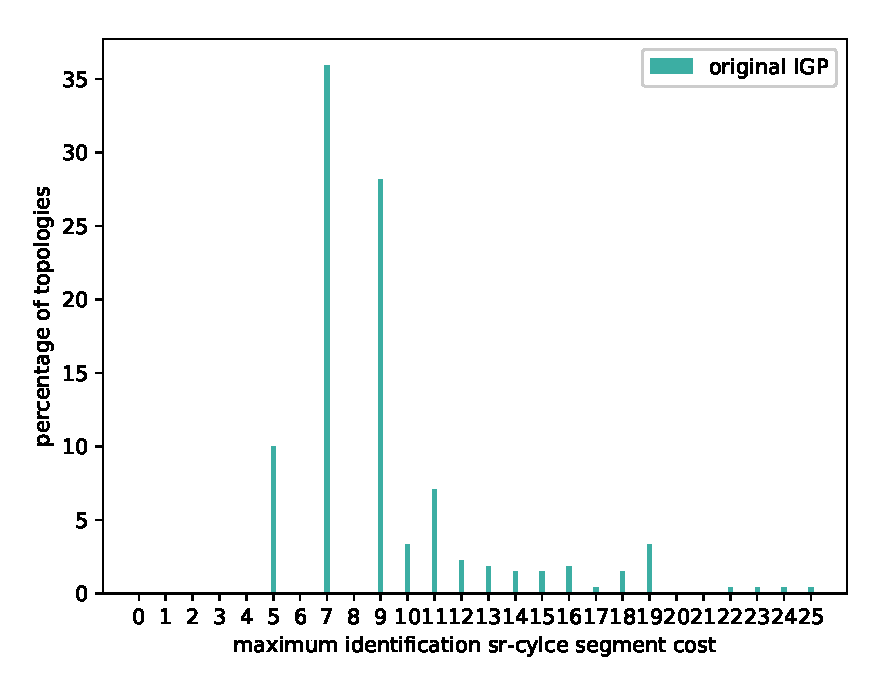
\includegraphics[width=.85\columnwidth]{./Network-lib/data/plot/minSegCover_identification_orig.eps}
\end{center}
\caption{Distribution of the maximum segment cost of the probing sr-cycles.}
\label{fig:min-seg-cost-segcost-orig}
\end{figure}


\begin{algorithm}[t]
\small
\caption{$\textsf{find-faulty-edge}\left( g, \sr{c} = \langle x_1, \ldots, x_l \rangle \right)$}
\begin{algorithmic}[1]
\STATE $c = (e_1, \ldots, e_n) \gets \seq(\sr{c})$
\STATE $L \gets 0, R \gets n$
\WHILE{$R - L \geq 2$}
  \STATE $i \gets \frac{L + R}{2}$
  \IF{$g.\textsf{isSymmetric}()$}
    \STATE $j \gets \min \ \left\{ j \in \{ 1, \ldots, l \} \mid e_i = x_j \vee \left(j < l \wedge e_i \in \sp(x^2_{j}, x^1_{j + 1})\right) \right\}$
    \IF{$e_i = x_j$}
      \STATE $\sr{c}_i \gets \langle x_1, \ldots, x_j, \rev(x_j), \ldots, \rev(x_1) \rangle$
    \ELSE
      \STATE $\sr{c}_i \gets \langle x_1, \ldots, x_{j - 1}, e^2_i, \rev(x_{j - 1}), \ldots, \rev(x_1) \rangle$
    \ENDIF
  \ELSE
    \STATE $\sr{c}_i \gets \textsf{min-segmentation}((e_1, \ldots, e_i, \rev(e_i), \ldots, \rev(e_1))$
  \ENDIF
  \STATE $\textit{status} \gets \textsf{send-probe}(\sr{c}_i)$
  \IF{$\textit{status} = \textit{received}$}
    \STATE $L \gets M$
  \ELSE
    \STATE $R \gets M$
  \ENDIF
\ENDWHILE
\IF{\textit{single-link failures}}
  \RETURN $e_L$
\ENDIF
\RETURN $\{ e_L, \rev(e_L) \}$
\end{algorithmic}
\label{algo:findedge}
\end{algorithm}

% 
% \subsection{Computing the cycle cover}
% 
% 
% \subsection{Min segment cost cycle cover}
% 
% \begin{lemma}
% \label{lemma:deterministic-concat2}
% Let $\sr{p} = \langle x_1 \ldots, x_l \rangle$ be a deterministic sr-path from $u_1$ to $u_2$ and 
% $\sr{q} = \langle y_1, \ldots, y_r \rangle$ be a sr-path from
% $v_1$ to $v_2$ such that $u_2 \neq v_1$ and $v_1 \in \nreach(u_2, 1)$. Then $\sr{p} \oplus \sr{q}$
% is a deterministic sr-path from $u_1$ to $v_2$ with 
% 
% \[ \cost(\sr{p} \oplus \sr{q}) =
%   \begin{cases}
%     \cost(\sr{p}) + \cost(\sr{q}) + 1 & \quad \text{if } y_1 \text{ is a node segment}\\
%     \cost(\sr{p}) + \cost(\sr{q})  & \quad \text{otherwise}
%   \end{cases}
% \]
% \end{lemma}
% 
% \begin{proof}
% The fact that $\sr{p} \oplus \sr{q}$ is deterministic is obvious since both $\sr{p}$ and $\sr{q}$ are deterministic and
% since $v_1 \in \nreach(u_2, 1)$ there is a unique shortest path connecting the last node of $\sr{p}$ to the first node of
% $\sr{q}$. Write $\sr{p} \langle x_1 \ldots, x_l \rangle$ and $\sr{q} = \langle y_1, \ldots, y_r \rangle$. If $y_i$ is a node
% segment, its cost is not included in $\sr{q}$ since it is the ingress node of that sr-path. However, it appears as a segment in 
% $\sr{p} \oplus \sr{q}$ since $u_2 \neq v_1$. Therefore in this case the segment cost in increased by $1$. Otherwise $y_i$ was already
% counted in $\cost(\sr{q})$ so the segment cost is just the sum of both costs. Note that the nature of $x_1$ does not matter as it remains
% the origin of the concatenation of the sr-paths.
% \end{proof}
% 
% \begin{lemma}
% \label{lemma:splitCost}
% Let $\sr{p} = \langle x_1, x_2, \ldots, x_l \rangle$. Then, for all $v \in V(G)$ and $i = 1, \ldots, l$ we have that
% $$
% \cost(\langle u, x_{i + 1}, \ldots, x_l \rangle) = \cost(\sr{p}) - \cost(\langle x_1, \ldots, x_i \rangle)
% $$
% \end{lemma}
% 
% \begin{proof}
% Since $u$ is a node segment, $\cost(\langle u, x_{i + 1}, \ldots, x_l \rangle) = \sum_{k = i + 1}^l \cost(x_k)$.
% On the other hand,
% \begin{align*}
% \cost(\sr{p}) - \cost(\langle x_1, \ldots, x_i \rangle) & = \sum_{k = 1}^l \cost(\sr{p}, x_i) - \sum_{k = 1}^i \cost(\sr{p}, x_i) \\
% & = \sum_{k = i + 1}^l \cost(\sr{p}, x_i) \\
% & = \cost(\langle u, x_{i + 1}, \ldots, x_l \rangle)
% \end{align*}
% \end{proof}
% 
% \begin{lemma}
% \label{lemma:splitCost2}
% Let $\sr{p} = \langle x_1, x_2, \ldots, x_l \rangle$, $i \in \{ 1, \ldots, l - 1 \}$, $k = \cost(\sr{p})$, $k_1 = \cost(\langle x_1, \ldots, x_i \rangle)$ 
% and $k_2 = \cost(\langle x_{i + 1}, \ldots, x_l \rangle)$. Then, 
% \[ k_2 =
%   \begin{cases}
%     k - k_1 - 1 & \quad \text{if } x_{i + 1} \text{ is a node segment}\\
%     k - k_1  & \quad \text{otherwise}
%   \end{cases}
% \]
% \end{lemma}
% 
% \begin{proof}
% We have that
% \begin{align*}
% k_2 & = \cost(\langle x_{i + 1}, \ldots, x_l \rangle) = \sum_{j = i + 1}^l \cost(x_j) \\
% \end{align*}
% If $x_{i + 1}$ is an adjacency segment then
% \end{proof}
% 
% 
% \begin{theorem}
% \label{thm:cyclecover}
% Let $G$ be a network, $s \in V(G)$ and $e \in E(G)$.
% There exists a deterministic sr-cycle $\sr{c}$ from $s$ to $s$ of segment cost at most $k$ covering $e = (u_1, u_2)$ if and only
% there exists $r \in \{0, \ldots, k\}$ such that one of these conditions holds
% \begin{enumerate}
%  \item $(u_1, u_2) \in \ereach(r, s)$ and $v \in \nreach(k - r, u_2)$
%  \item there exists $x \in \nreach(r, s)$ and $y \in \nreach(x, 1)$ such that $e \in \sp(x, y)$ and $s \in \nreach^n(k - r - 1, y)$
%  \item there exists $x \in \nreach(r, s)$ and $y \in \nreach(x, 1)$ such that $e \in \sp(x, y)$ and $s \in \nreach^e(k - r, y)$
% \end{enumerate}
% \end{theorem}
% 
% \begin{proof}
% $(\Rightarrow)$ Suppose that $c = \langle x_1, \ldots, x_l \rangle$ is a deterministic sr-cycle from $s$ to $s$ of segment cost at most $k$ covering $e$.
% Since $c$ covers $e$, there exists the smallest $i$ such that $\langle x_1, \ldots, x_i \rangle$
% covers edge $e$.
% 
% \emph{Case 1:} $x_i = e$: Write $r = \cost(\langle x_1, \ldots, x_i \rangle)$. Then, by Lemma \ref{lemma:splitCost},
% $\langle u_2, x_{i + 1}, \ldots, x_l \rangle$ is a sr-path of cost at most $k - r$ from $u_2$ to
% $s$. Hence $s \in \nreach(k - r, u_2)$.
% 
% \emph{Case 2:} $x_i \neq e$: Then, by choice of $i$, $e$ belongs to the unique shortest path betweeh $x^2_{i - 1}$ and $x^1_{i}$.
% Let $x = x^2_{i - 1}$, $y = x^1_i$ and $r = \cost(\langle x_1, \ldots, x_{i - 1} \rangle)$. 
% Then, since $c$ is deterministic, $x = x^2_{i - 1} \in \nreach(s, r)$ and $y = x^1_i \in \nreach(1, x)$.
% If $x_i$ is a node segment then $\langle x_{i + 1}, \ldots, x_l \rangle$ has cost $k - r - 1$ so $s \in \nreach^n(k - r - 1, y)$.
% Otherwise, $\langle x_{i + 1}, \ldots, x_l \rangle$ has cost $k - r$ so $s \in \nreach^e(k - r, y)$. Since $e \in \sp(x, y)$ we 
% see that either condition $2.$ or $3.$ from the above theorem is satisfied.
% 
% $(\Leftarrow)$ Suppose that there exists $r$ such that $(u_1, u_2) \in \ereach(v, r)$ and $v \in \nreach(u_2, k - r)$.
% There there exists a sr-path $\sr{p}$ from $v$ to $u_2$ covering $e$ of segment cost at most $r$ and 
% a sr-path $\sr{q}$ from $u_2$ to $v$ of segment cost at most $k - r$. By Lemma \ref{lemma:deterministic-concat},
% $\sr{c} = \sr{p} \oplus \sr{q}$ is a deterministic sr-cycle from $v$ to $v$ covering edge $e$ with $\cost(\sr{c}) \leq r + k - r = k$
% 
% Suppose now that there exists $x \in \nreach(v, r)$ and $y \in \nreach(x, 1)$ such that $e \in \sp(x, y)$ and $v \in \nreach(y, k - r)$.
% Then there exists a sr-path $\sr{p}$ from $v$ to $x$ with $\cost(\sr{p}) \leq r$ and a sr-path $\sr{q}$ from $y$ to $v$
% with $\cost(\sr{q}) \leq k - r$. Since $y \in \nreach(x, 1)$, by Lemma \ref{lemma:deterministic-concat2} \todo{this lemma does not exists, concatenation of
% paths not ending in the same node but with unique shoretest path between}, $\sr{c} = \sr{p} \oplus \sr{q}$ is a deterministic sr-cycle
% from $v$ to $v$ with $\cost(\sr{c}) \leq r + k - r = k$. Since $e \in \sp(x, y)$ this cycle covers $e$.
% \end{proof}


\section{Dual topology monitoring}
\label{section:complete-igp}

As we showed before, the minimum number of segments required to cover a topology can be quite high.
One idea to reduce it is to have a separate set of IGP weights. The ones already configured on the network used
to forward traffic and new ones that are used only for sending the monitoring probes.

One idea to compute those weights would be to first compute a minimum cycle cover of the network using
some standard existing algorithm \cite{FAN1992113} (note that here we are talking about cycles, not 
sr-cycles). Then we could compute a set of weights such that the maximum number of segments required to
segment any of those cycles is as small as possible. We did not solve this problem and therefore leave
it as an open problem (with a slightly more general formulation).

\begin{problem}{Optimal segmentation IGP}
Given a graph $G$ and a set $P$ of paths on $G$ compute a IGP weight function 
$\igp : E(G) \rightarrow \mathbb{N}$ such that if we compute a minimal segmentation
of every path $p \in P$ whose maximum segment cost amongst those sr-paths is minimal.
\end{problem}

We believe that solving this problem could be very useful in any setting where having a dual weight
topology is infeasible in practice. This would be yet another way to leverage existing graph theory to solve the 
problem and then translate those graph theoretic solutions into segment routing solutions with low
segment cost.

Another possibility, which we explore in this thesis, is to compute a set of $\igp$ weights such that 
there is a unique shortest path between any pair of nodes \emph{and} every edge belongs to a unique shortest
path. The intuition of why this will make segmentations less costly is that the conditions for needing to add
a new segment in the minimum segmentation algorithm is exactly the existence of multiple shortest paths or
an edge that does not belong to any shortest path.
Note that our two conditions cannot both coexist in a network with parallel links. With two links between
$u$ and $v$, we cannot have at the same time that both those links belong to some shortest path and a unique
shortest path between $u$ and $v$. We therefore relax the definition as follows.

\begin{definition}
Let $G$ be a graph. A set of IGP weights $\igp : E(G) \rightarrow \mathbb{N}$ is said to be
\emph{complete} if and only if for all $u, v \in V(G)$ at least one edge of $E(G, u, v)$ belong to a shortest path.
\end{definition}

\begin{definition}
Let $G$ be a graph. A set of IGP weights $\igp : E(G) \rightarrow \mathbb{N}$ is said to be
\emph{ECMP-free} if and only if for all $u, v \in V(G)$ there is a unique shortest path between $u$ and $v$.
\end{definition}

\subsection{Computing ECMP-free and complete IGP weights}

\begin{definition}
Let $G$ be a graph. A set of IGP weights $\igp : E(G) \rightarrow \mathbb{N}$ is said to be
\emph{total} if and only all simple paths on $G$ have a different weight.
\end{definition}

Computing a total weighting of a graph $G$ is trivial. We can simply set $\igp(e) = 2^{\idx(e)}$ for
all $e \in E(G)$. Since $\idx(e)$ assigns a unique index between $0$ and $|E(G)| - 1$ to the edges
of $G$, this IGP function will assign a different power of two to each edge of $G$. Therefore,
any two distinct simple paths must have a different IGP weight since those weights will
correspond to sums of distinct powers of $2$.

The following lemma shows, unsurprisingly, that one way to build ECMP-free weights is to compute
total weights.

\begin{lemma}
\label{lemma:totalToECMP}
Let $G$ be a graph. If $\igp : E(G) \rightarrow \mathbb{N}$ is total then it is ECMP-free.
\end{lemma}

\begin{proof}
Trivial from the definition. Any shortest path is simple and thus any two shortest paths must 
have a different IGP weight since $\igp$ is total.
\end{proof}

The following result shows that we can transform any total IGP weighting $\igp$ into a complete one by
adding a large enough constant. This constant can by any value above the maximum between the diameter of the
graph with respect to $\igp$ and the maximum weight of any edge. Being larger than the diameter ensures
that shortest paths remain unique and being larger than the maximum weight ensures that every edge belong to a shortest path. 
The diameter of a network is the greatest distance (in terms of number of edges)
between any pair of vertices.

\begin{lemma}
\label{lemma:totalToComplete}
Let $G$ be a network. Let 
$$
M \geq \max \left( diam(G, \igp), \displaystyle \max_{e \in E(G)} \igp(e) \right).
$$
Then, if $\igp : E(G) \rightarrow \mathbb{N}$ is total then 
$\igp^+ : E(G) \rightarrow \mathbb{N}$ defined by $\igp^+(e) = \igp(e) + M$ is complete.
\end{lemma}

\begin{proof}
Let $p_1 = (e_1, \ldots, e_n)$ and $p_2 = (f_1, \ldots, f_m)$ be two paths on $G$. 

We start by proving that $\igp^+(p_1) \neq \igp^+(p_2)$. By definition
$\igp^+(p_1) = \igp(p_1) + n \cdot M$ and $\igp^+(p_2) = \igp(p_2) + m \cdot M$. By hypothesis, 
$\igp(p_1) \neq \igp(p_2)$ Assume without loss of generality that $\igp(p_1) > \igp(p_2)$. If $n = m$ then
\begin{align*}
\igp^+(p_1) = \igp(p_1) + n \cdot M > \igp(p_2) + n \cdot M = \igp(p_2) + m \cdot M = \igp^+(p_2).
\end{align*}
By definition of $M$, we have $M \geq diam(G, \igp) \geq \igp(p_1), \igp(p_2) > 0$. Thus, if $n > m$ then,
\begin{align*}
\igp^+(p_1) & = \igp(p_1) + n \cdot M > n \cdot M \geq (m + 1) \cdot M \\
& = M + m \cdot M \geq \igp(p_2) + m \cdot M = \igp^+(p_2)
\end{align*}
Similarly, if $n < m$ then
\begin{align*}
\igp^+(p_2) & = \igp(p_2) + m \cdot M > m \cdot M \geq (n + 1) \cdot M \\
& = M + n \cdot M \geq \igp(p_1) + n \cdot M = \igp^+(p_1).
\end{align*}
Thus, in any case, $\igp^+(p_1) \neq \igp^+(p_2)$. We conclude that $\igp^+$ is total
and therefore also ECMP-free.

Let $u, v \in V(G)$. We now show that at least one edge $e \in E(G, u, v)$ belongs to a shortest path with respect to $\igp^+$.
Let $e \in E(G, u, v)$ be such that $\igp(e)$ is minimum. Since $\igp$ is total, this edge is unique. 
By Proposition \ref{prop:sp-properties}, $e$ belongs to a shortest path if and only if $e$ is a shortest path between
$u$ and $v$. Suppose that $e$ is not a shortest path for $\igp^+$. Then there exists a path $p = (e_1, \ldots, e_n)$ from $u$ to $v$ such that
$\igp^+(p) < \igp(e)$. Since $e$ is the unique edge between $u$ and $v$ of minimum cost, $n \geq 2$. By definition of $M$, we have $M \geq \igp(e)$ so 
\begin{align*}
\igp^+(p) = \igp(p) + n \cdot M \geq \igp(p) + 2 \cdot M > 2 \cdot M \geq 2 \cdot \igp(e) > \igp(e).
\end{align*}
This contradicts the fact that $e$ is not a shortest path for $\igp^+$. Therefore $\igp^+$ is complete.
\end{proof}

\begin{corollary}
Let $G$ be a graph and $\igp : E(G) \rightarrow \mathbb{N}$ defined such that
$$
\igp(e) = 2^{\idx(e)} + 2^{|E(G)|}.
$$
Then $\igp$ is ECMP-free and complete.
\end{corollary}

\begin{proof}
We have already observed that $e \mapsto 2^{\idx(e)}$ is total and thus ECMP-free by Lemma \ref{lemma:totalToECMP}. Completeness then follows from
Lemma \ref{lemma:totalToComplete} by observing that 
$$
2^{|E(G)|} = \left( \sum_{e \in E(G)} 2^{\idx(e)} \right) + 1 > \max \left( diam(G, \igp), \displaystyle \max_{e \in E(G)} \igp(e) \right).
$$
\end{proof}

The problem with these IGP weights is that they are exponential with respect to the number of edges in the graph.
In practice IGP weights are represented with a $16$-bit integer and thus is maximum value is $2^{16} - 1 = 65535$.
This makes them useless in practice since they can only be implemented on a network with at most $15$ edges.

This motivates the following problem.

\begin{problem}{Minimum weight complete weighting}
\label{prob:minComplete}
\textbf{Input:} A network $G$.

\textbf{Output:} A complete and ECMP-free weighting $\igp : E(G) \rightarrow \mathbb{N}$ such that
$\displaystyle \max_{e \in E(G)} \igp(e)$ is minimum.
\end{problem}

Any approach for solving Problem \ref{prob:minComplete} that is based on Lemma \ref{lemma:totalToComplete} is domed to fail.
To see why this is true consider $\mathcal{K}_n$, the complete graph on $n$ nodes. It is not hard to see that $\mathcal{K}_n$ 
contains an exponential number of simple paths. 

%Any simple path on $\mathcal{K}_n$ corresponds to a sequence of nodes
%of length at most $n - 1$ without repetitions. Therefore, the number of such paths is
%$$
%P = \frac{1}{2} \sum_{l = 2}^n \frac{n!}{(n - l)!} \approx \frac{en!}{2}.
%$$

Any permutation of $n$ elements corresponds to a simple path on $\mathcal{K}_n$ 
of length $n - 1$ and there are $n!$ permutations of $n$ elements. Since a total weight must assign a different weight to
\emph{every} simple path, this shows that a total weight on the complete graph $\mathcal{K}_n$ will be such that at least
one simple path of length $n - 1$ has a weight of at least $n!$. Therefore this path must contain one edge of weight
$\frac{n!}{n - 1}$ since otherwise the total weight of the path would be lower than $n!$.

This shows that total weightings require exponential weights on any graph with an exponential number of paths. Most graphs
have an exponential number of simple paths with respect to its size. Hence, using Lemma \ref{lemma:totalToComplete} is bound
to provide weights that are very high. In contrast, it is not hard to see that $e \mapsto 1$ is an ECMP-free and complete weighting of
$\mathcal{K}_n$. This shows that such exponential bounds do not apply for the weight that we are looking for, only for total ones.

If we only care about the practical applicability of the weights, we can relax Problem \ref{prob:minComplete} into the following one.

\begin{problem}{Implementable complete weighting}
\label{prob:implemComplete}
\textbf{Input:} A network $G$.

\textbf{Output:} A complete and ECMP-free weighting $\igp : E(G) \rightarrow \mathbb{N}$ such that
$\displaystyle \max_{e \in E(G)} \igp(e) \leq 2^{16} - 1$.
\end{problem}

\subsection{Prime-based complete IGP}

We propose a partial solution to Problem \ref{prob:implemComplete}. Our solution is able to find a solution for $97.7\%$ of the instances in our dataset.
Let $m = |E(G)|$ be the number of edges in the graph and $\mathbb{P}_m = \{ \pi_0, \ldots, \pi_{m - 1} \}$ a set of $m$ prime numbers such that
$\pi_i \leq \pi_{i + 1}$. It is well known that two sets of distinct prime numbers
have a different product. Our idea is based on the fact that $\log(x \cdot y) = \log(x) \cdot \log(y)$. If we could set any real valued IGP weights,
one solution would be to use $e \mapsto \log(\pi_{\idx(e)})$ because the unicity of products between prime numbers would translate into unique sums
and thus unique path weights. To simplify the notations, we write $\pi_e$ instead of $\pi_{\idx(e)}$.
In this way, by what we observe above, two distinct paths would necessarily have distinct IGP costs.

Since we need integers we will use truncated logarithms instead. These logarithms are defined as
$$
\lnt{s}(x) = \lfloor 10^s \cdot \ln(x) \rfloor.
$$
For instance, $\lnt{4}(5) = \lfloor 10^4 \cdot 1.60943 \rfloor = 16094$. The idea is, starting from $s = 1$, to grow $s$ 
until the IGP weights defined by $e \mapsto \lnt{s}(\pi_e)$ are ECMP-free. A priori, nothing guarantees that doing so will 
eventually achieve it but we will prove shortly that it does. Since we also want the IGP weights to also be complete, we use
a slight different set of IGP weights $\igp^s : E(G) \rightarrow \mathbb{N}$ defined as $\igp^s(e) = \lnt{s}(\pi_e) + \lnt{s}(\pi_m)$.
The intuition behind the addition of the largest $\lnt{s}(\pi_m)$ term for achieving completeness is similar to the addition of the constant $M$
from Lemma \ref{lemma:totalToComplete}. We now prove that by growing $s$, $\igp^s$ eventually becomes ECMP-free and complete.

  
\begin{proposition}
\label{prop:converge}
Let $A$ and $B$ be two distinct subsets of $\mathcal{P}_m$, $P = \prod_{x \in \mathcal{P}_x} x$ and $q \in \mathcal{P}_m$. If $s > \log_{10} \left( 2 m \cdot q^m P \right)$, 
then 
$$
\sum_{x \in A} \left( \overline{\ln}^s(x) + \overline{\ln}^s(q) \right) \neq \sum_{x \in B} \left( \overline{\ln}^s(x) + \overline{\ln}^s(q) \right).
$$
\end{proposition}

\begin{proof}
Given any $s$ and $X \subseteq \mathcal{P}_m$, we have
\begin{equation}
\small
\label{eq:lg}
10^s \cdot \ln \left( \prod_{x \in X} x \right) \geq \sum_{x \in X} \overline{\ln}^s(x) \geq 10^s \cdot \ln \left( \prod_{x \in X} x \right) - |X|
\end{equation}

Let $q \in \mathcal{P}_m$. Write $a = \prod_{x \in A} x$ and $b = \prod_{x \in B} x$. Assume without loss of generality that $q^{|A|} a > q^{|B|} b$ (they are not equal because they contain distinct prime numbers). 
Then by (\ref{eq:lg})
\begin{align*}
\tiny
\sum_{x \in A} \overline{\ln}^s(x) +  \overline{\ln}^s(q) & \geq \sum_{x \in A} 10^s \ln(x q) - 2 \geq \\
& 10^s \ln(q^{|A|} a) - 2 |A|
\end{align*}
and $\sum_{x \in B} \overline{\ln}^s(x) + \overline{\ln}^s(q) \leq 10^s \ln (q^{|B|} b)$. Therefore
\begin{align*}
\tiny
\sum_{x \in A} \overline{\ln}^s(x) +  \overline{\ln}^s(q) - \sum_{x \in B} \overline{\ln}^s(x) + \overline{\ln}^s(q) & \geq \\
10^s \ln(q^{|A|} a) - 2 |A| - 10^s \ln (q^{|B|} b) & \geq \\
10^s  \ln \left(q^{|A|} a \slash q^{|B|} b \right) - 2 |A| \geq & \\
10^s  \ln \left(q^{|A|} a \slash (q^{|A|} a - 1) \right) - 2 |A| \geq & \\
10^s \slash (q^{|A|} a) - 2|A| \geq 10^s \slash (q^m P) - 2m
\end{align*}
Which is positive as long as $s > \log_{10} \left( 2 m \cdot q^m P \right)$.
\end{proof}

\begin{corollary}
If $s > \log_{10} \left( 2 m \cdot q^m P \right)$ then $\igp^s$ is ECMP-free.
\end{corollary}

\begin{proof}
Let $p_1, p_2$ be two paths on $G$ and $q = \pi_m$. By Proposition \ref{prop:converge}, 
$$
\igp^s(p_1) = \sum_{e \in E(p_1)} \left( \overline{\ln}^s(e) + \overline{\ln}^s(\pi_m) \right) \neq \sum_{e \in E(p_2)} \left( \overline{\ln}^s(e) + \overline{\ln}^s(\pi_m) \right) = \igp^s(p_2).
$$
Therefore $\igp^s$ is total and thus, by Lemma \ref{lemma:totalToComplete}, this means that 
it will also be ECMP-free.
\end{proof}

\begin{proposition}
The weights $\igp^s$ are complete for any $s \geq 1$.
\end{proposition}

\begin{proof}
Let $u, v \in V(G)$. Assume that the shortest path $p$ from $u$ to $v$ is not a single edge.
Let $e$ be any edge between $u$ and $v$. Then,
\begin{align*}
\tiny
w(p) & = |E(p)| \cdot \overline{\ln}^s(\pi_m) + \sum_{e \in E(P)} \overline{\ln}^s(\pi_e) > |E(p)| \cdot \overline{\ln}^s(\pi_m) \geq \\
& 2 \cdot \overline{\ln}^s(\pi_m) \geq \overline{\ln}^s(\pi_e) + \overline{\ln}^s(\pi_m) = w(e)
\end{align*}
Therefore $p$ cannot be a shortest path proving that $\igp^s$ is complete.
\end{proof}

These results provide a theoretical guarantee that the above mentioned process will eventually converge towards 
ECMP-free and complete weights. However, even for small graphs the value of $\log_{10} \left( 2 m \cdot q^m P \right)$ is
large and thus, if $s > \log_{10} \left( 2 m \cdot q^m P \right)$, then $10^s$ will be really huge. But this a theoretical bound on how long we need to wait to reach a \emph{total} function.
But we do not care about totality, we only want ECMP-freeness (completeness is true for any $s$). Therefore, our algorithm
will iterate over $s$ and, at each step, check whether ECMP-freeness holds with the hope that this will occur a long time before
totality occurs. Our experiments show that this is indeed the case. Figure \ref{fig:primeIGP_s} shows the distribution of the
value of $s$ over all topologies from out dataset. We can see that this value is indeed much smaller than the theoretical bound.

\begin{figure}
\begin{center}
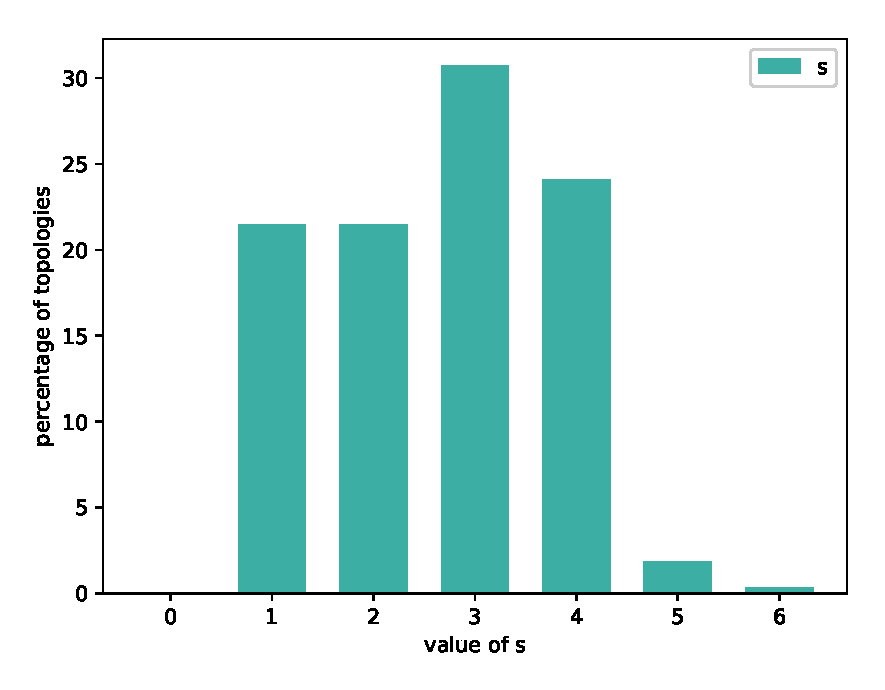
\includegraphics[width=.85\columnwidth]{./Network-lib/data/plot/primeIGP_s.eps}
\end{center}
\caption{Distribution, over all topologies, of the exponent $s$ required for $\igp^s$ to be ECMP-free and complete.}
\label{fig:primeIGP_s}
\end{figure}

We analyzed the percentage of topologies for which this process results in weights that go above the maximum configurable value $2^{16} - 1$.
It turns out that for this happens only for $2.3\%$ of the topologies as show in the CDF in Figure \ref{fig:primeIGP}. The threshold value
is shown with a dotted line.

\begin{figure}
\begin{center}
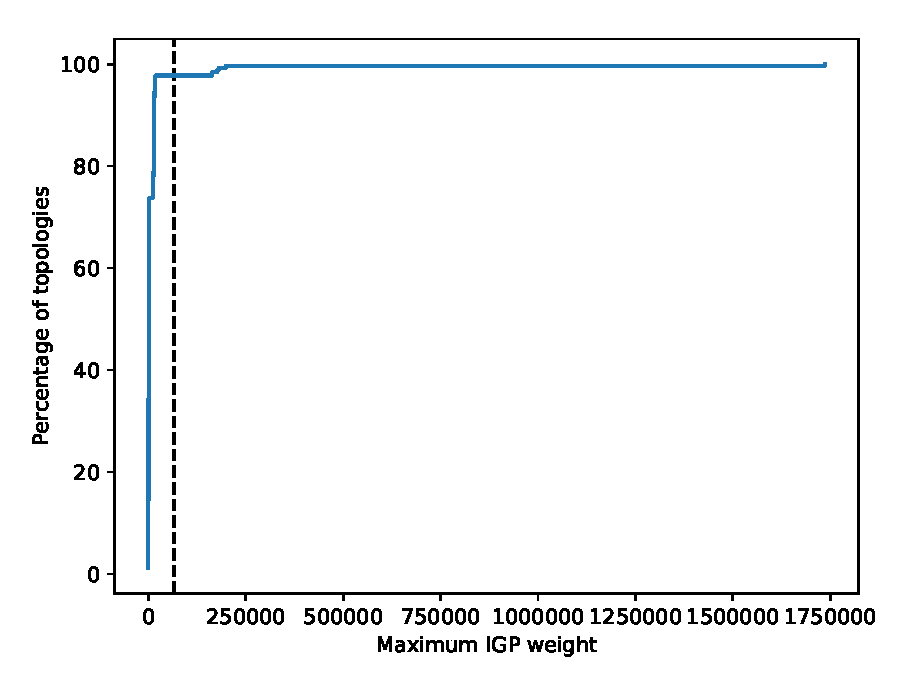
\includegraphics[width=.85\columnwidth]{./Network-lib/data/plot/primeIGP.eps}
\end{center}
\caption{CDF of maximum weight obtained over all topologies.}
\label{fig:primeIGP}
\end{figure}

Algorithm \ref{algo:primeIGP} provides a pseudo-code implementation of this algorithm described above.
The first step of the algorithm is to compute a set of $m = |E(G)|$ prime numbers. We can find these by iterating over the integers $2, 3, 5, 7, 9, \ldots$
and using any primality test algorithm to check which ones are prime numbers. The Prime number theorem \cite{Cormen:2009:IAT:1614191} %page 888 theorem 31.37
tells us that the $m$-th prime number is close to $m \cdot \ln(m)$ so we find them in a small number of steps.
This is not the most efficient way to achieve this but since $m$ is relatively small it is fast enough for our purposes.

\begin{algorithm}[t]
\small
\caption{$\textsf{primeIGP}\left( G \right)$}
\begin{algorithmic}[1]
%\algrule
\cmtline{compute the first $|E(G)|$ primes}
\STATE $m \gets |E(G)|$
\STATE $\mathcal{P} \gets \{ 2 \}$
\STATE $p \gets 3$
\WHILE{$|\mathcal{P}| < m$}
  \IF{$\textsf{isPrime}(p)$}
    \STATE $\mathcal{P} \gets \mathcal{P} \cup \{p\}$
  \ENDIF
  \STATE $p \gets p + 2$
\ENDWHILE
\cmtline{initialize weights}
\STATE $f \gets 1$
\FOR{$e \in E(G)$}
  \STATE $w(e) \gets \lfloor f \cdot \log(p_e) \rfloor + \lfloor f \cdot \log(p_m) \rfloor$
\ENDFOR
\cmtline{iterate until weights converge}
\WHILE{\textbf{not} $\textsf{ECMP-free}(w)$ \textbf{or not} $\textsf{complete}(w)$}
  \STATE $f \gets 10 \cdot f$
  \FOR{$e \in E(G)$}
    \STATE $w(e) \gets \lfloor f \cdot \log(p_e) \rfloor + \lfloor f \cdot \log(p_m) \rfloor$
  \ENDFOR
\ENDWHILE
\RETURN $w$
\end{algorithmic}
\label{algo:primeIGP}
\end{algorithm}

\subsection{Randomized complete IGP}

In practice, there seems to be a much simpler solution for generating relatively small ECMP-free and complete IGP weights.
We performed some experiments that showed that random weighs tend to be ECMP-free as long as the maximum value is not too small.
Therefore, a solution for generating ECMP-free weights that are also complete is to randomly generate weights for each edge 
and then adding the maximum generated weight to each edge to guarantee completeness. Algorithms \ref{algo:randomIGP} and \ref{algo:randomw}
formalize this process. Note that without the step of adding the maximum weight, our experiments showed that the algorithm
has a low probability of success. This is normal because otherwise there is no control over the weight of a single edge 
and so it can easily happen that it is assigned a high value making it impossible for it to belong to a shortest path.

\begin{algorithm}[t]
\small
\caption{$\textsf{randomIGP}\left( G, M \right)$}
\begin{algorithmic}[1]
%\algrule
\STATE $w \gets \textsf{random-w}(G, M)$
\WHILE{\textbf{not} $\textsf{ECMP-free}(w)$ \textbf{or not} $\textsf{complete}(w)$}
  \STATE $w \gets \textsf{random-w}(G, M)$ 
\ENDWHILE
\RETURN $w$
\end{algorithmic}
\label{algo:randomIGP}
\end{algorithm}

\begin{algorithm}[t]
\small
\caption{$\textsf{random-w}\left( G, M \right)$}
\begin{algorithmic}[1]
%\algrule
\FOR{$e \in E(G)$}
  \STATE $w(e) \gets \textsf{random}(1, \ldots, M)$
\ENDFOR
\FOR{$e \in E(G)$}
  \STATE $w'(e) \gets w(e) + \max_{e \in E(G)} w(e)$
\ENDFOR
\RETURN $w'$
\end{algorithmic}
\label{algo:randomw}
\end{algorithm}

In practice we tried it over all topologies with $M = 100$ for each of them we found a solution on average in at most $2$ iterations (over $100$ runs).
For this reason, in practice we strongly recommend using this simple algorithm. However we were unable to prove any bound on the probability of success
of this algorithm. Hence we cannot say whether it will work well beyond our dataset. We leave the following problem as another interesting open problem.

\begin{lemma}
For any network $G$ and $M \in \mathbb{N}$ the weight function produced by Algorithm \ref{algo:randomw} is complete. 
\end{lemma}

\begin{proof}
Let $w$ be the random weights produced by the algorithm after the first loop and $w'$ the final weights. Let $M = \max_{e \in E(G)} w(e)$. 
Let $u, v \in V(G)$ and $p$ be a path from $u$ to $v$ with at least two edges.
Then
$$
w'(p) = w(p) + |E(p)| \cdot M > 2 \cdot M \geq w(e) + M = w'(e)
$$
for any edge $e \in E(G)$. Therefore the shortest path between $u$ and $v$ must be a single edge $e \in E(G, u, v)$.
\end{proof}

\begin{problem}{Randomized weighting}
\label{prob:randomIGP}
\textbf{Input:} A network $G$ and a integer constant $M \in \mathbb{N}$. 

\textbf{Output:} The probability that $\textsf{random-w}\left( G, M \right)$ outputs an ECMP-free IGP weight function.
\end{problem}

\subsection{Cycle covers with ECMP-free and complete IGP}

In this section we evaluate the benefits of using ECMP-free and complete IGP weights.
We start by evaluating the minimum number of segments required in a minimum segment cost
sr-cycle cover. Recall that Algorithm \ref{algo:min-seg-cover2} computes a sr-cycle cover such
that the maximum number of segments in any sr-cycle is as small as possible. In Figure 
\ref{fig:min-seg-cover-segcost} we already evaluated the segment cost of the solutions obtained 
by this algorithm over the original IGP weights. Figure \ref{fig:min-seg-cost-segcost-new} shows
the distribution of the segment costs with and without special IGP weights. We observe that ECMP-free
and complete weights obtain the desired effect of greatly reducing the segment cost of minimum
cost sr-cycle covers. For $100\%$ of the topologies we need sr-cycles with segment cost at most $4$ whereas before
about $55\%$ of the topologies required sr-cycles with segment cost $5$ or more.

\begin{figure}
\begin{center}
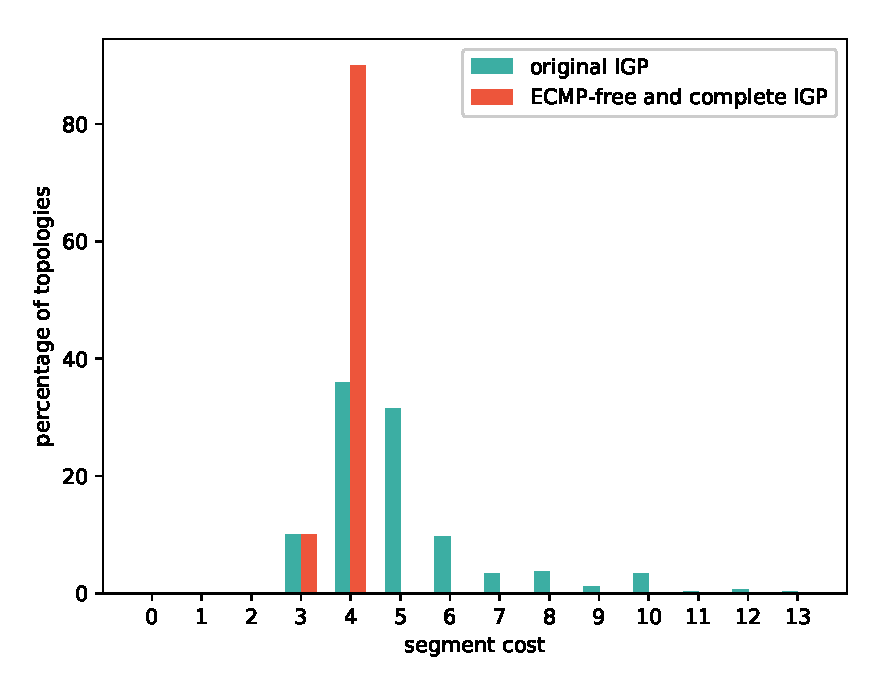
\includegraphics[width=.85\columnwidth]{./Network-lib/data/plot/minSegCover_segcost_complete.eps}
\end{center}
\caption{Distribution of the maximum segment cost of the probing sr-cycles with and without ECMP-free and complete weights.}
\label{fig:min-seg-cost-segcost-new}
\end{figure}

Next we analyze the benefits of using special IGP weights with respect to the segment cost of the 
identification sr-cycles. Recall that our network monitoring solution uses probing sr-cycles to periodically
check whether every link is still up and one identification sr-cycles to pinpoint a failure when
a monitoring probe fails to return to the vantage point. Figure \ref{fig:min-seg-cost-segcost-new}
shows how much do we gain in terms of segment cost by having ECMP-free and complete IGP weights. We can see that
using these weights makes it possible to implement such a monitoring scheme on a lot more networks since the maximum
number of segments required becomes $9$ rather than the original high value of $19$.

\begin{figure}
\begin{center}
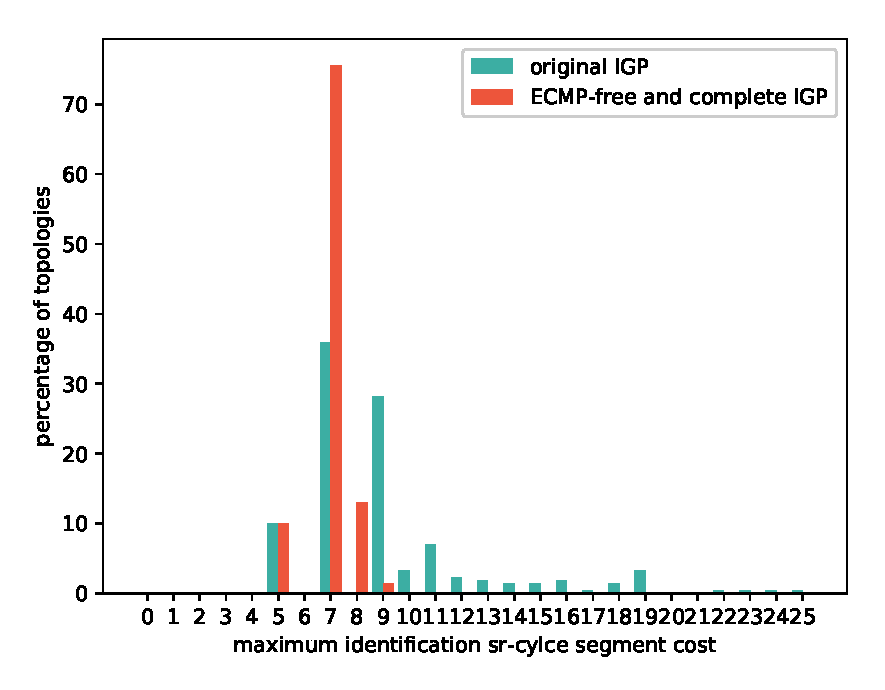
\includegraphics[width=.85\columnwidth]{./Network-lib/data/plot/minSegCover_identification.eps}
\end{center}
\caption{Distribution of the maximum segment cost of the identification sr-cycles with and without ECMP-free and complete weights.}
\label{fig:min-seg-cost-segcost-new}
\end{figure}


\section*{Conclusion}

In this chapter we proposed a solution for identifying single-link failures in a network.
We showed that even if multiple failures occur, our algorithm can still identify a pair of 
edges $e$, $\rev(e)$ such that one of them is faulty with certainty.

Our experiments show that our algorithm runs in a reasonable amount of time considering that
these cycles need to be installed only once in the network. 

Our solution works on the original topology and prides the theoretical minimum number of segments
required to implement any cycle cover using segment routing. This was achieved by using our reachability
theory developed in Chapter \ref{chapter:sr}. We also showed that if this segment cost
is too high, we can reduce it by working with a dual topology maxing the whole network monitoring 
process cost at most $9$ segments in the worst case, over all topologies from out dataset.

This was a second example where column generation provides good results when applied to solve an
segment routing optimization problem.
